% Options for packages loaded elsewhere
% Options for packages loaded elsewhere
\PassOptionsToPackage{unicode}{hyperref}
\PassOptionsToPackage{hyphens}{url}
\PassOptionsToPackage{dvipsnames,svgnames,x11names}{xcolor}
%
\documentclass[
]{agujournal2019}
\usepackage{xcolor}
\usepackage{amsmath,amssymb}
\setcounter{secnumdepth}{5}
\usepackage{iftex}
\ifPDFTeX
  \usepackage[T1]{fontenc}
  \usepackage[utf8]{inputenc}
  \usepackage{textcomp} % provide euro and other symbols
\else % if luatex or xetex
  \usepackage{unicode-math} % this also loads fontspec
  \defaultfontfeatures{Scale=MatchLowercase}
  \defaultfontfeatures[\rmfamily]{Ligatures=TeX,Scale=1}
\fi
\usepackage{lmodern}
\ifPDFTeX\else
  % xetex/luatex font selection
\fi
% Use upquote if available, for straight quotes in verbatim environments
\IfFileExists{upquote.sty}{\usepackage{upquote}}{}
\IfFileExists{microtype.sty}{% use microtype if available
  \usepackage[]{microtype}
  \UseMicrotypeSet[protrusion]{basicmath} % disable protrusion for tt fonts
}{}
\makeatletter
\@ifundefined{KOMAClassName}{% if non-KOMA class
  \IfFileExists{parskip.sty}{%
    \usepackage{parskip}
  }{% else
    \setlength{\parindent}{0pt}
    \setlength{\parskip}{6pt plus 2pt minus 1pt}}
}{% if KOMA class
  \KOMAoptions{parskip=half}}
\makeatother
% Make \paragraph and \subparagraph free-standing
\makeatletter
\ifx\paragraph\undefined\else
  \let\oldparagraph\paragraph
  \renewcommand{\paragraph}{
    \@ifstar
      \xxxParagraphStar
      \xxxParagraphNoStar
  }
  \newcommand{\xxxParagraphStar}[1]{\oldparagraph*{#1}\mbox{}}
  \newcommand{\xxxParagraphNoStar}[1]{\oldparagraph{#1}\mbox{}}
\fi
\ifx\subparagraph\undefined\else
  \let\oldsubparagraph\subparagraph
  \renewcommand{\subparagraph}{
    \@ifstar
      \xxxSubParagraphStar
      \xxxSubParagraphNoStar
  }
  \newcommand{\xxxSubParagraphStar}[1]{\oldsubparagraph*{#1}\mbox{}}
  \newcommand{\xxxSubParagraphNoStar}[1]{\oldsubparagraph{#1}\mbox{}}
\fi
\makeatother


\usepackage{longtable,booktabs,array}
\usepackage{calc} % for calculating minipage widths
% Correct order of tables after \paragraph or \subparagraph
\usepackage{etoolbox}
\makeatletter
\patchcmd\longtable{\par}{\if@noskipsec\mbox{}\fi\par}{}{}
\makeatother
% Allow footnotes in longtable head/foot
\IfFileExists{footnotehyper.sty}{\usepackage{footnotehyper}}{\usepackage{footnote}}
\makesavenoteenv{longtable}
\usepackage{graphicx}
\makeatletter
\newsavebox\pandoc@box
\newcommand*\pandocbounded[1]{% scales image to fit in text height/width
  \sbox\pandoc@box{#1}%
  \Gscale@div\@tempa{\textheight}{\dimexpr\ht\pandoc@box+\dp\pandoc@box\relax}%
  \Gscale@div\@tempb{\linewidth}{\wd\pandoc@box}%
  \ifdim\@tempb\p@<\@tempa\p@\let\@tempa\@tempb\fi% select the smaller of both
  \ifdim\@tempa\p@<\p@\scalebox{\@tempa}{\usebox\pandoc@box}%
  \else\usebox{\pandoc@box}%
  \fi%
}
% Set default figure placement to htbp
\def\fps@figure{htbp}
\makeatother


% definitions for citeproc citations
\NewDocumentCommand\citeproctext{}{}
\NewDocumentCommand\citeproc{mm}{%
  \begingroup\def\citeproctext{#2}\cite{#1}\endgroup}
\makeatletter
 % allow citations to break across lines
 \let\@cite@ofmt\@firstofone
 % avoid brackets around text for \cite:
 \def\@biblabel#1{}
 \def\@cite#1#2{{#1\if@tempswa , #2\fi}}
\makeatother
\newlength{\cslhangindent}
\setlength{\cslhangindent}{1.5em}
\newlength{\csllabelwidth}
\setlength{\csllabelwidth}{3em}
\newenvironment{CSLReferences}[2] % #1 hanging-indent, #2 entry-spacing
 {\begin{list}{}{%
  \setlength{\itemindent}{0pt}
  \setlength{\leftmargin}{0pt}
  \setlength{\parsep}{0pt}
  % turn on hanging indent if param 1 is 1
  \ifodd #1
   \setlength{\leftmargin}{\cslhangindent}
   \setlength{\itemindent}{-1\cslhangindent}
  \fi
  % set entry spacing
  \setlength{\itemsep}{#2\baselineskip}}}
 {\end{list}}
\usepackage{calc}
\newcommand{\CSLBlock}[1]{\hfill\break\parbox[t]{\linewidth}{\strut\ignorespaces#1\strut}}
\newcommand{\CSLLeftMargin}[1]{\parbox[t]{\csllabelwidth}{\strut#1\strut}}
\newcommand{\CSLRightInline}[1]{\parbox[t]{\linewidth - \csllabelwidth}{\strut#1\strut}}
\newcommand{\CSLIndent}[1]{\hspace{\cslhangindent}#1}



\setlength{\emergencystretch}{3em} % prevent overfull lines

\providecommand{\tightlist}{%
  \setlength{\itemsep}{0pt}\setlength{\parskip}{0pt}}



 


\usepackage{url} %this package should fix any errors with URLs in refs.
\usepackage{lineno}
\usepackage[inline]{trackchanges} %for better track changes. finalnew option will compile document with changes incorporated.
\usepackage{soul}
\linenumbers
\makeatletter
\@ifpackageloaded{caption}{}{\usepackage{caption}}
\AtBeginDocument{%
\ifdefined\contentsname
  \renewcommand*\contentsname{Table of contents}
\else
  \newcommand\contentsname{Table of contents}
\fi
\ifdefined\listfigurename
  \renewcommand*\listfigurename{List of Figures}
\else
  \newcommand\listfigurename{List of Figures}
\fi
\ifdefined\listtablename
  \renewcommand*\listtablename{List of Tables}
\else
  \newcommand\listtablename{List of Tables}
\fi
\ifdefined\figurename
  \renewcommand*\figurename{Figure}
\else
  \newcommand\figurename{Figure}
\fi
\ifdefined\tablename
  \renewcommand*\tablename{Table}
\else
  \newcommand\tablename{Table}
\fi
}
\@ifpackageloaded{float}{}{\usepackage{float}}
\floatstyle{ruled}
\@ifundefined{c@chapter}{\newfloat{codelisting}{h}{lop}}{\newfloat{codelisting}{h}{lop}[chapter]}
\floatname{codelisting}{Listing}
\newcommand*\listoflistings{\listof{codelisting}{List of Listings}}
\makeatother
\makeatletter
\makeatother
\makeatletter
\@ifpackageloaded{caption}{}{\usepackage{caption}}
\@ifpackageloaded{subcaption}{}{\usepackage{subcaption}}
\makeatother
\usepackage{bookmark}
\IfFileExists{xurl.sty}{\usepackage{xurl}}{} % add URL line breaks if available
\urlstyle{same}
\hypersetup{
  pdftitle={Adaptive Introgression Shapes the Pan-genome of Populus Hybrid Zones},
  pdfauthor={Baxter Worthing},
  colorlinks=true,
  linkcolor={blue},
  filecolor={Maroon},
  citecolor={Blue},
  urlcolor={Blue},
  pdfcreator={LaTeX via pandoc}}



\draftfalse

\begin{document}
\title{Adaptive Introgression Shapes the Pan-genome of Populus Hybrid
Zones}

\authors{Baxter Worthing\affil{1}}
\affiliation{1}{The University of Vermont, }



\begin{abstract}
Poplar trees\ldots{}
\end{abstract}





\subsection{Introduction}\label{introduction}

Hybridization can lead to the exchange of genetic variation across
species boundaries, a process known as introgression. Introgression is a
powerful source of genetic novelty, playing a significant role in the
evolutionary history of natural systems (Hedrick, 2013; Suarez-Gonzalez,
Lexer, et al., 2018), humans (Racimo et al., 2015) and key crop
varietals (Burgarella et al., 2019; Cheng et al., 2019; Gao et al.,
2019; Kou et al., 2020; Qiao et al., 2021; Sun et al., 2020; Zanini et
al., 2022). Admixed individuals, the recipients of introgressed
sequence, harbor novel combinations of alleles originating from both
parental species, and may present phenotypic variation which transcends
that observed in the parental species. In this sense, admixed
individuals represent unique opportunities, not only to better
understand the genetic basis of phenotype, but also to better understand
the nature of molecular interactions between divergent haplotypes.
Furthermore, when parental species inhabit differing environments,
patterns of introgression may also reflect the interaction between
genetic variation and environment. Ultimately, these GxG and GxE
interactions define the contexts in which introgression is adaptive.
Past research on natural admixed populations suggests that introgression
can be an adaptive process, through which genetic variation related to
locally-adaptive phenotypes is passed from one species to another
(Gaczorek et al., 2024; Hamilton \& Miller, 2016; Hedrick, 2013; Kremer
\& Hipp, 2020; Leroy et al., 2020; Rendón-Anaya et al., 2021; Savolainen
et al., 2007; Suarez-Gonzalez, Lexer, et al., 2018). Closer and more
extensive analysis of natural manifestations of adaptive introgression
can reveal the types of genetic variation that are able to cross species
boundaries without a fitness consequence, the regions of the genome that
are receptive to the introduction of foreign sequence, and the degree to
which environmental context influences the adaptive nature of
introgression. Research in this area is valuable not only because it
sheds light on important questions in evolutionary biology, such as the
evolution of species boundaries and molecular basis of adaptive traits,
but also because it gauges the overall potential for the introduction of
divergent genetic variation into novel genetic and environmental
background. Therefore, research in this area has great potential for
broader impact for two main reasons. First, because the contribution of
biotechnology to advances in the fields of medicine and agriculture
increasingly depend on the introduction of genetic sequence into a novel
background. Second, because introgression provides a potentially faster
and more reliable route for the adaptive evolution of phenotype than de
novo mutation, meaning that natural systems and breeding programs alike
may depend on introgression in order to facilitate rapid evolution of
adaptive traits in response to changing climates.

The size and molecular origin of the genetic variation that is exchanged
between species through adaptive introgression is important to define,
as a growing body of research suggests that genomic structural variation
(SV), here defined as genetic variation larger than 50bp resulting for
insertion, deletion, translocation or inversion of genomic sequence, is
often the causal variation underlying ecologically and economically
important traits in many taxa (\emph{CITE}). For instance, SV may play a
role in local adaptation to climate, and past research shows divergence
between populations for SV genotypes resulting from local adaptation
(Hämälä et al., 2021; Y. Li et al., 2024; Z. Li et al., 2023;
Songsomboon et al., 2021). At a broader scale, research also shows that
SV maintain genetic differentiation between species (Ferguson et al.,
2024; L. Zhang et al., 2021). However, little is known about the
adaptive exchange of SV genotypes between divergent populations and
species. Introgression between crop varietals and wild relatives is a
key factor in the breeding history of many crops, and recent work shows
that SV are often the causal variants involved in this process (Cheng et
al., 2019; Gao et al., 2019; Kou et al., 2020; Qiao et al., 2021; Sun et
al., 2020,; Zanini et al., 2022). Introgression is also common in
natural systems and recent work highlights introgression as an important
source of adaptive genetic novelty in many species, particularly forest
trees (Hamilton \& Miller, 2016; Leroy et al., 2020; Rendón-Anaya et
al., 2021; Suarez-Gonzalez, Lexer, et al., 2018). However, past work on
the genetics of such adaptive introgression in natural systems focused
primarily on SNP genotypes. While hybrid genomes may be porous to
variation at the single nucleotide scale, and introgressed SNP alleles
may even present an adaptive advantage in admixed individuals, it
remains unclear if the same is true for SV genotypes, which have greater
potential for deleterious phenotypic effects. Recently, research has
highlighted a potential role for SV in adaptive introgression. This work
suggests that SV may play an important role in both adaptive
introgression (Almarri et al., 2020; Xia et al., 2023; X. Zhang et al.,
2021) and in the maintenance of species boundaries (L. Zhang et al.,
2021). If SV is indeed involved in adaptive introgression, it is worth
investigating the molecular nature (eg size, frequency, variant class,
genomic location) of the SV alleles involved, as well as the consistency
and directionality of adaptive introgression involving SV. Admixed
individuals may present mosaics of SV alleles derived from both parental
species, or introgression may be directionally biased toward one
species. Similarly, some loci may act as barriers to introgression,
while others are more receptive. Natural hybrid zones may be hotspots
for the de novo generation of SV alleles through processes such as
unequal crossing over. Here, we leverage extensive sampling of natural
forest tree hybrid zones, cutting edge techniques for genotyping SV in
admixed individuals and established landscape genomics analyses to
investigate these areas of uncertainty.

The study of SV in natural hybrid zones is challenging, as it requires
the ability to accurately genotype SV in a large number of admixed
individuals. The majority of past research on SV in natural hybrid zones
has relied on the use of reference genomes derived from a single
individual from only one of the parental species, which can lead to
reference bias (Bock et al., 2023; Feng et al., 2024; Song et al.,
2023). Reference bias occurs when the genomes of resequenced individuals
contain regions that are highly diverged from the reference genome
sequence, causing reads originating from these regions to align
incorrectly, or not align at all. This can lead to misinterpretation or
under-representation of variation resulting from admixture (Secomandi et
al., 2025). Reference bias is particularly problematic when studying SV,
as large insertions and deletions may be longer than sequencing reads,
making variation in their presence and absence (PAV) challenging to
detect. Furthermore, SV is often species-specific and, because admixed
individuals represent a mixture of genetic variation from two or more
species, the presence of reference bias can obscure the effect that the
presence (or absence) of genetic variation has on traits, and can hinder
the identification of SV that is involved in introgression.

Recently, an increasing number of studies have relied on pan-genome
assembly to overcome reference bias and to accurately genotype SV (Gao
et al., 2019; Kang et al., 2023; Y. Li et al., 2024; Z. Li et al., 2023;
Liang et al., 2025; Secomandi et al., 2025; Songsomboon et al., 2021). A
pan-genome assembly is a non-redundant collection of sequences
originating from multiple individuals. This genetic information can be
represented as ``nodes'' in a pan-genome graph, while the linear
sequence of each input genome is stored as a ``path'' connecting a
series of nodes. In a pan-genome graph, each node describes the
alignment between at least two sequences, given an expected level of
sequence divergence (Kang et al., 2023). Pan-genome graphs can capture
complex variation that is not present in a single reference genome, and
can provide a more accurate representation of the genetic variation
present in admixed individuals. Pan-genome assembly has been used to
identify and genotype SV related to ecologically and economically
important traits in a variety of taxa, and has been shown to be an
effective tool for studying adaptive evolution in natural populations
(Fang \& Edwards, 2024; Kang et al., 2023; Secomandi et al., 2025).
Pan-genome assembly could help overcome the challenges of studying SV in
admixed tree populations, and could provide new insights into the role
of SV in adaptive introgression in natural populations of forest trees
(Secomandi et al., 2025). Despite this potential, we know of only one
study that used pan-genome assembly to examine introgression in the
context of hybridization in the wild. Liang et al.~(2025) use a
pan-genome based approach to genotype SV in a range-wide sampling of the
interfertile oak species \emph{Quercus variabilis} and \emph{Q.
acutissima}, showing that SV harbor signals of adaptive introgression
that differ from those detected from SNP data and identifying adaptive
introgression of SV genotypes in a gene rich region of oak chromosome 9
(Liang et al., 2025). In light of this work, it is worth investigating
if signatures adaptive introgression on SV exist in other interfertile
tree species and asking not only how this adaptive signal is distributed
across the whole genome but also how it varies with environmental
context across the range of hybridizing species. Here, we add to this
nascent line of research by leveraging pan-genome assembly and
fine-scale sampling of natural hybrid zones to explore genome-wide
relationship between structural variation and introgression between
\emph{Populus balsamifera} and \emph{Populus trichocarpa}, two forest
tree species that diverged much more recently than the oak species
studied by Liang et al.~(2025).

\emph{Populus balsamifera} and \emph{Populus trichocarpa} readily
interbreed in nature, and early and advanced generation hybrids have
been described in hybrid zones located where their ranges overlap
(Chhatre et al., 2018; Geraldes et al., 2014; Suarez-Gonzalez et al.,
2016; Suarez-Gonzalez, Hefer, et al., 2018). It is thought that
hybridization between these two species facilitates introgression of
genetic variation related to locally-adaptive phenotypes from one
species to the other (Suarez-Gonzalez et al., 2016; Suarez-Gonzalez,
Hefer, et al., 2018). However, studies on controlled inter-specific
crosses in \emph{Populus} have made it clear that introgression is often
biased toward particular regions of the genome, particular
\emph{Populus} species, or specific environments (Lexer et al., 2005;
Meirmans et al., 2017; Thompson et al., 2010). Therefore, the porosity
of the genome to adaptive introgression between these species may be
constrained by incompatibilities between the genomic variants involved
as well as environmental context, two factors which warrant further
investigation. The environmental context of adaptive introgression may
be of particular importance in the case of \emph{P. balsamifera} and
\emph{P. trichocarpa}. \emph{P. balsamifera} is more commonly found in
colder, continental climates while \emph{P. trichocarpa} is more often
associated with milder, coastal climates with longer growing seasons
(Geraldes et al., 2014; Suarez-Gonzalez, Hefer, et al., 2018).
Considering hybrid zones between these species often fall along the
boundaries of their ranges (Chhatre et al. (2018); Fetter \& Keller
(2023)), it seems possible that adaptive introgression helps hybrid
individuals persist in environments that are outside of the optimum for
either parental species. Suarez-Gonzalez, Hefer, et al. (2018) showed
support for this hypothesis, finding that introgressed regions in the
genomes of hybrids harbored signs of selection and variation associated
with adaptive traits, including phenology. However, the specific
adaptive variants within these genomic regions, and the nature of their
effects on fitness remain, for the most part, undiscovered.
Identification of SV involved in adaptive introgression between these
two species would not only contribute to a broader understanding of the
molecular basis of adaptive introgression, but would also provide
helpful insight into the conservation of these ecologically important
species. In trees, long generations times are thought to limit the
potential contribution of de novo mutation to adaptive evolution in
response to rapid environmental change (Feng et al., 2024; Savolainen et
al., 2007). Therefore, adaptive introgression is viewed as one of the
few routs for speicies like \emph{P. balsamifera} and \emph{P.
trichocarpa} to adaptively evolve in response to climate change (Feng et
al., 2024). If adaptive introgression does help admixed individuals
persist in environments outside of their optimum, then the variation
involved could guide genetic conservation efforts, such as assisted gene
flow. Furthermore, industrial breeding of \emph{Populus} varietals
generally involves interspecific crosses, and breeding programs would
benefit from a clearer understanding of the genetic variation that is
involved in adaptive introgression between these two species.

Here, we take advantage of recent advances in pan-genome assembly
methods to produce a pan-genome reference, comprising 24 diverse
haplotypes from \emph{P. balsamifera}, \emph{P. trichocarpa} and their
hybrids, facilitating unbiased analysis of the sequence variation that
is segregating within natural \emph{Populus} hybrid zones. Using this
new pan-genome assembly, we genotype structural variation across 566
individuals sampled from within and outside of 6 distinct \emph{P.
balsamifera} and \emph{P. trichocarpa} hybrid zones. We assess the
extent of genomic diversity present in these species and their hybrids,
identifying genomic variation that is not present in the \emph{P.
trichocarpa} reference genome. Furthermore, we describe structural
variation involved both in introgression and in genomic divergence
between the two species. We shed light on the role that introgression
may play in shaping the pan-genome of these species, and the degree to
which tree genomes are porous to the inter-specific exchange of
structural variant alleles.

\subsection{Methods}\label{methods}

\subsubsection{Sample collection and whole genome
sequencing}\label{sample-collection-and-whole-genome-sequencing}

In January 2020, we collected dormant branch cuttings from 546 poplar
trees along 7 distinct latitudinal transects spanning natural contact
zones between Populus trichocarpa and Populus balsamifera
Figure~\ref{fig-1}. Short read whole genome sequencing and subsequent
bioinformatic analyses were performed as described in Bolte et
al.~(2024). Briefly, Genomic DNA libraries for all sampled individuals
were constructed at the Duke University Center for Genomic and
Computational Biology and sequenced using an Illumina NovaSeq 6000
instrument with an S4 flow cell with 64 samples per lane (Illumina Inc.,
San Diego, USA). De-indexing, QC, trimming adapter sequences, and
sequence pre-processing were completed by the sequencing facility. In
addition to short read sequencing, we also sequenced a subset of 40
sampled individuals with PacBio HiFi long reads. We harvested tissue
from newly-expanded leaves grown under low light conditions to use for
high molecular weight DNA extraction. After confirming extraction
quality through gel electrophoresis and bioanalysis, we submitted HMW
DNA to the University of Maryland Center for Integrative Biosciences
Genomics Core Facility for library preparation and sequencing on the the
PacBio Sequel system with two samples per SMRT flow cell. We sequenced
one \emph{P. balsamifera} sample (939) for an additional run on a full
SMRT cell. We also sequenced this individual with Oxford Nanopore
Technology (ONT) platform. We submitted high molecular weight DNA to the
Vermont Integrative Genomics Resource Sequencing Center for library
preparation and sequencing on XXX flowcell (two runs) and XXX flowcell
(one run)

\subsubsection{Genome assembly}\label{genome-assembly}

Of the 40 individuals sequenced with HiFi long reads, we selected 16 for
whole genome assembly Figure~\ref{fig-1}. These samples ranged from 20
to 35x long read coverage. We performed de-novo genome assembly of the
HiFi reads for these samples with HiCanu (Nurk et al., 2020). We set
HiCanu parameters as follows: gSize=``400m'', lc=``5'', lcer=``0.055'',
ovrlp=``350'', mincov=``9''. To detect potential contaminants in the raw
assemblies produced by HiCanu, we used the program Kraken2 to compare
the k-mer content of assembled contigs to the ``PlusPFP'' database of
known taxon-specific k-mers representing archaea, bacteria, viral,
human, protozoa, fungi and plant taxa (Lu et al., 2022). We then used a
custom bioawk script to remove any assembled contig that Kraken2
assigned to a taxonomic unit other than \emph{Populus}, leaving only
unassigned or \emph{Populus}- assigned contigs in each assembly. We
assessed the accuracy and completeness of the decontaminated assemblies
using QUAST and BUSCO (Gurevich et al., 2013; Simão et al., 2015). To
further assess the contiguity and quality of these assemblies, we used
minimap2 and BWA to map the original HiFi reads and additional Illumina
short reads back to each assembled haplotype (H. Li, 2018; H. Li \&
Durbin, 2010). We passed these alignments to the program CRAQ (K. Li et
al., 2023), which leverages read depth along assembled contigs for
quality assessment. We repeated these quality assessment checks at each
subsequent stage of genome assembly. Phasing, or the separation and
concatenation of contigs belonging to the same parental haplotype is a
key step in genome assembly for hybrid individuals, as divergent
haplotypes likely contain important genetic information. We used
mininmap2 to map reads back to assembled contigs and to map assembled
contigs to themselves. We then used the purge haplotigs pipeline (Roach
et al., 2018) to split diploid assemblies into two assembled haploytpes
for each individual. We used RagTag (Alonge et al.~2022) to connect
decontaminated, phased contigs into pseudo-chromosomal scaffolds, guided
by alignments of assembled contigs to the Nisqually1 \emph{P.
trichocarpa} reference genome. We visually inspected minimap2 alignments
of scaffolded assemblies to the reference genome to identify potential
scaffolding errors. We used RepeatMasker to annotate and mask repetitive
regions and annotated possible coding domains and predicted protein
sequences for each assembly with AUGUSTUS (Smit et al., 2015; Hoff et
al., 2019).

\subsubsection{Pan-genome assembly}\label{pan-genome-assembly}

In a pan-genome graph, a non-redundant collection of all input sequences
is represented as ``nodes'', while the linear sequence of each input
genome is stored as a ``path'' connecting a series of nodes. In this
approach to graph construction, each node of the graph w describes the
alignment between at least two sequences, given an expected level of
sequence divergence. We constructed a pan-genome graph from an all-by
all alignment of the 24 assembled haplotypes. Any contigs shorter than
100kb were dropped before alignment. We used wfmash (Guarracino et al.,
2021) to perform all-by-all alignments between assembled chromosomes,
and seqwish (Garrison and Guarracino, 2022) to project alignments into a
graph pan-genome assembly. Pan-genome graphs constructed this way can
have highly complex topography, which may hinder downstream applications
such a sequence alignment. To combat this issue, we used the program
smoothXG to smooth complex variation in these graphs. We also assembled
a separate graph specifically for subsequent alignment-based analyses
using the minigraph-cactus pipeline (Hickey et al., 2023). We used the
program panacus to asses pan-genome growth and coverage statistics
(Parmigiani et al., 2024). We used the program ODGI (Guarracino et al.,
2022) to perform basic graph quality control and to partition the core (
sequence present in all individuals), shell (sequence variably present
or absent across individuals) and singleton sequence (present in only
one individuals) content for each graph and individual represented in
the graphs. We used the program vg (Garrison et al., 2018) to
deconstruct each graph assembly into a VCF containing the variation
encapsulated in each graph. We passed this deconstructed VCF file to
vcfbub (github.com/pangenome/vcfbub) to collapse nested SV sites into
the top-level variant for all SV less than 10kb in length. Using
bcftools (Danecek et al., 2021) we split biallelic sites into
multiallelic records for this deconstructed vcf.

\subsubsection{Genotyping Pan-genomic
Variation}\label{genotyping-pan-genomic-variation}

We aligned sequencing reads from additional samples to pan-genome graph
assembly to genotype SNPs and SVs. We aligned PacBio HiFi reads for 40
total individuals (including the 16 used to construct the pan-genome
graph) to the minigraph-cactus graph using the program GraphAligner
(Rautiainen \& Marschall, 2020). To characterize sequence variation
across a broader set of individuals, we also mapped Illumina short reads
for 575 individuals to the pan-genome graph using the program giraffe
(Sirén et al., 2021). We then called SV and SNPs from these alignments
using the vg call algorithm (Garrison et al., 2018). We used bcftools to
split multialleleic calls into separate records, normalize alleles
against the \emph{P. trichocarpa} reference and merge calls for all
samples into one VCF representing SV and SNP genotypes in the \emph{P.
trichocarpa} reference coordinate space.

\subsubsection{Analysis of Structural Variation and
Introgression}\label{analysis-of-structural-variation-and-introgression}

We used ADMIXTURE results from Bolte et al (2024) to assign each
individual an admixture proportion at K=2 and K=4. The genetic data used
for this ADMIXTURE analysis came from SNP calls from mappings of the
same illlumina reads used in this study, however they were mapped to the
\emph{P. trichocarpa} reference genome. We used this same genetic data
set to perform local ancestry inference (LAI) using LOTR (Dias-Alves et
al., 2018). These ADMIXTURE and LAI data sets were used to visualize and
analyze patterns of local and global genomic ancestry throughout this
study.

We used ODGI to flatten the Nisqually1 \emph{P. trichocarpa} reference
genome path in the cactus graph. We then used a bed file representation
of this path and reference gene annotations to genotype PAV of reference
sequence across all paths of the cactus graph. We used R version 4.1.0
to identify core and shell gene sequences from this data and to perform
PCA on the PAV genotypes (R Core Team, 2024). We also ran a similar PAV
PCA with the merged vcf representing all 575 sequenced samples in this
study, using plink2 (Chang et al., 2015). We used the
-\/--allele-weights flag to extract the loading of each allele for each
SV on the first 3 principal components.

To find SV potentially involved in introgression, we employed custom
scripts to identify ancestry blocks along the chromosomes of all 335
admixed individuals in this study. An individual was considered admixed
if its k=2 ADMIXTURE score indicated at least 5 percent admixture
genome-wide. We used Bedtools (Quinlan \& Hall, 2010) to find SV that
overlapped ancestry blocks in each admixed individual. We then scored
each SV allele based on its prevalence in ancestry blocks that
contrasted the average global ancestry of an individual.

For all SV that were outliers in principal component or LAI analyses, we
used Bedtools to check for overlap with annotated genes. We then used
plantgenie to analyze PFAM enrichment of gene sets (Sundell et al.,
2015).

\subsection{Results}\label{results}

\subsubsection{Whole genome sequencing and
assembly.}\label{whole-genome-sequencing-and-assembly.}

Illumina sequencing yielded on average of 8358 MB of sequence,
corresponding to an average sequencing depth of 21x. PacBio HiFi
sequencing yielded on average 6368 MB of sequence, corresponding to an
average sequencing depth of 16x. Sample 939 was sequenced to a depth of
roughly 60X HiFi and roughly 20X ONT reads. Table 1 shows summary
statistics for the 16 whole genome assemblies included in the
pan-genome. Assembly quality and contiguity were generally high, however
alternate haplotypes were not always fully assembled (Table 1).

\subsubsection{Pan-genome assembly}\label{pan-genome-assembly-1}

The minigraph-cactus pangenome graph contained a total of 102,907,131
nodes comprising 1.2 Gbp of sequence. Of this, 243 Mbp was present
across all individuals (core genome), while 423Mbp was present in some
but not all individuals (shell genome). The remaining 537 Mbp
represented singleton sequence. Figure~\ref{fig-2} shows how the size of
the sequence classes changes as individuals are added to the pan-genome.
Figure~\ref{fig-3} shows the proportions of core, shell and singleton
sequence within each sample. \textbf{?@fig-4} shows each genome in the
pan-genome graph plotted on the first two principal components of a PCA
on PAV of reference sequence.

\subsubsection{Pan-genomic Variation}\label{pan-genomic-variation}

3708 annotated genes were variably present or absent across the 17
genomes used to construct the pan- =genome. These genes were
significantly enriched for various protein families including NB-ARC
domain, D-mannose binding lectin, sulfotransferases, cupins, and
Cytochrome P450. Of these shell genes, 167 were present in all of the
pure \emph{P. trichocarpa} individuals and none of the pure \emph{P.
balsamifera} samples making up the pan-genome graph. These \emph{P.
trichocarpa} - specific genes were enriched for protein families,
including sulfotransferases, serine carboxypeptidases, Mlo family
proteins, D-mannose binding lectin, Glycosyl hydrolases and absistic
acid (ABA) induced proteins.

The cactus pan-genome graph contained 1,773,427 SV greater than 20bp in
length. Figure~\ref{fig-5} shows the distribution of these variants
across the genome. The distribution of frequencies of the non-reference
allele for these SV is shown in Figure~\ref{fig-6}.

The first two principal components of a PCA on PAV genotyped from short
read alignments to the pan-genome graph are shown in Figure~\ref{fig-7}.
The loading of each allele for each SV on the first principal component
of a PCA on PAV genotyped from short read alignments to the pan-genome
graph is shown in \textbf{?@fig-8}. The SV that were outliers on PC1
overlapped 1362 annotated genes. These genes were significantly enriched
for protein families involved in development and growth (K-Box proteins,
KNOX proteins), cold tolerance (DEAD/DEAH box helicases), and phenology
(SRF transcription factors).

\subsubsection{SV and Introgression}\label{sv-and-introgression}

We identified 126,973 SV that overlapped ancestry blocks in admixed
individuals, and found that 30,721 of these were associated with blocks
of either \emph{P. trichocarpa} or \emph{P. balsamifera} ancestry in
admixed individuals.

\subsubsection{Tables}\label{tables}

\pandocbounded{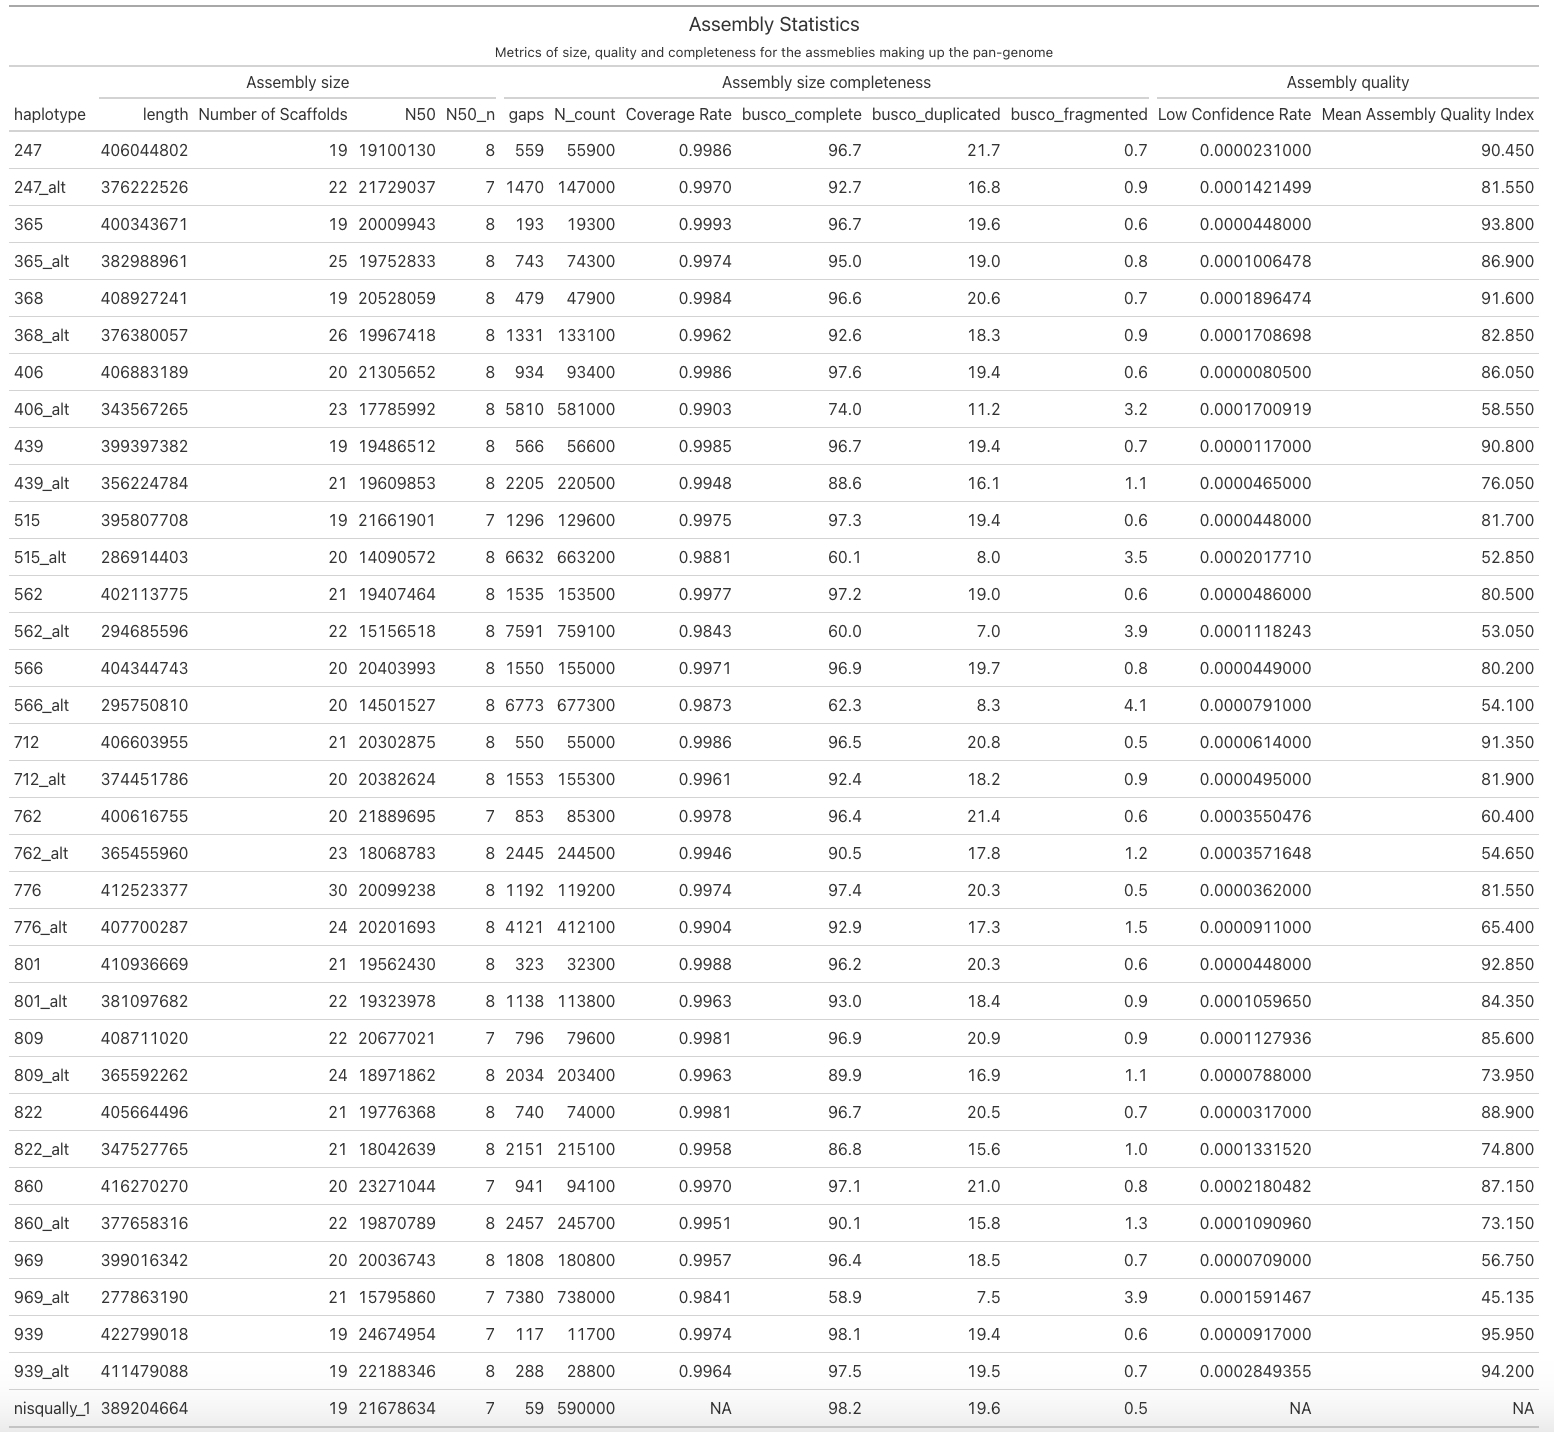
\includegraphics[keepaspectratio]{figs/table.jpg}}\{fig-format:
svg\}

\section{Figures}\label{figures}

\begin{figure}

\begin{minipage}{0.50\linewidth}

\centering{

\pandocbounded{\includegraphics[keepaspectratio]{figs/msamp.jpg}}

}

\subcaption{\label{fig-1a}}

\end{minipage}%
%
\begin{minipage}{0.50\linewidth}

\centering{

\pandocbounded{\includegraphics[keepaspectratio]{figs/msamp_sub.jpg}}

}

\subcaption{\label{fig-1b}}

\end{minipage}%

\caption{\label{fig-1}(a): sampling locations for 575 individuals used
in this study, color indicates ancestry based in ADMIXTURE analysis (b):
A subset of 16 individuals used for whole genome assembly}

\end{figure}%

\begin{figure}

\begin{minipage}{0.50\linewidth}

\centering{

\pandocbounded{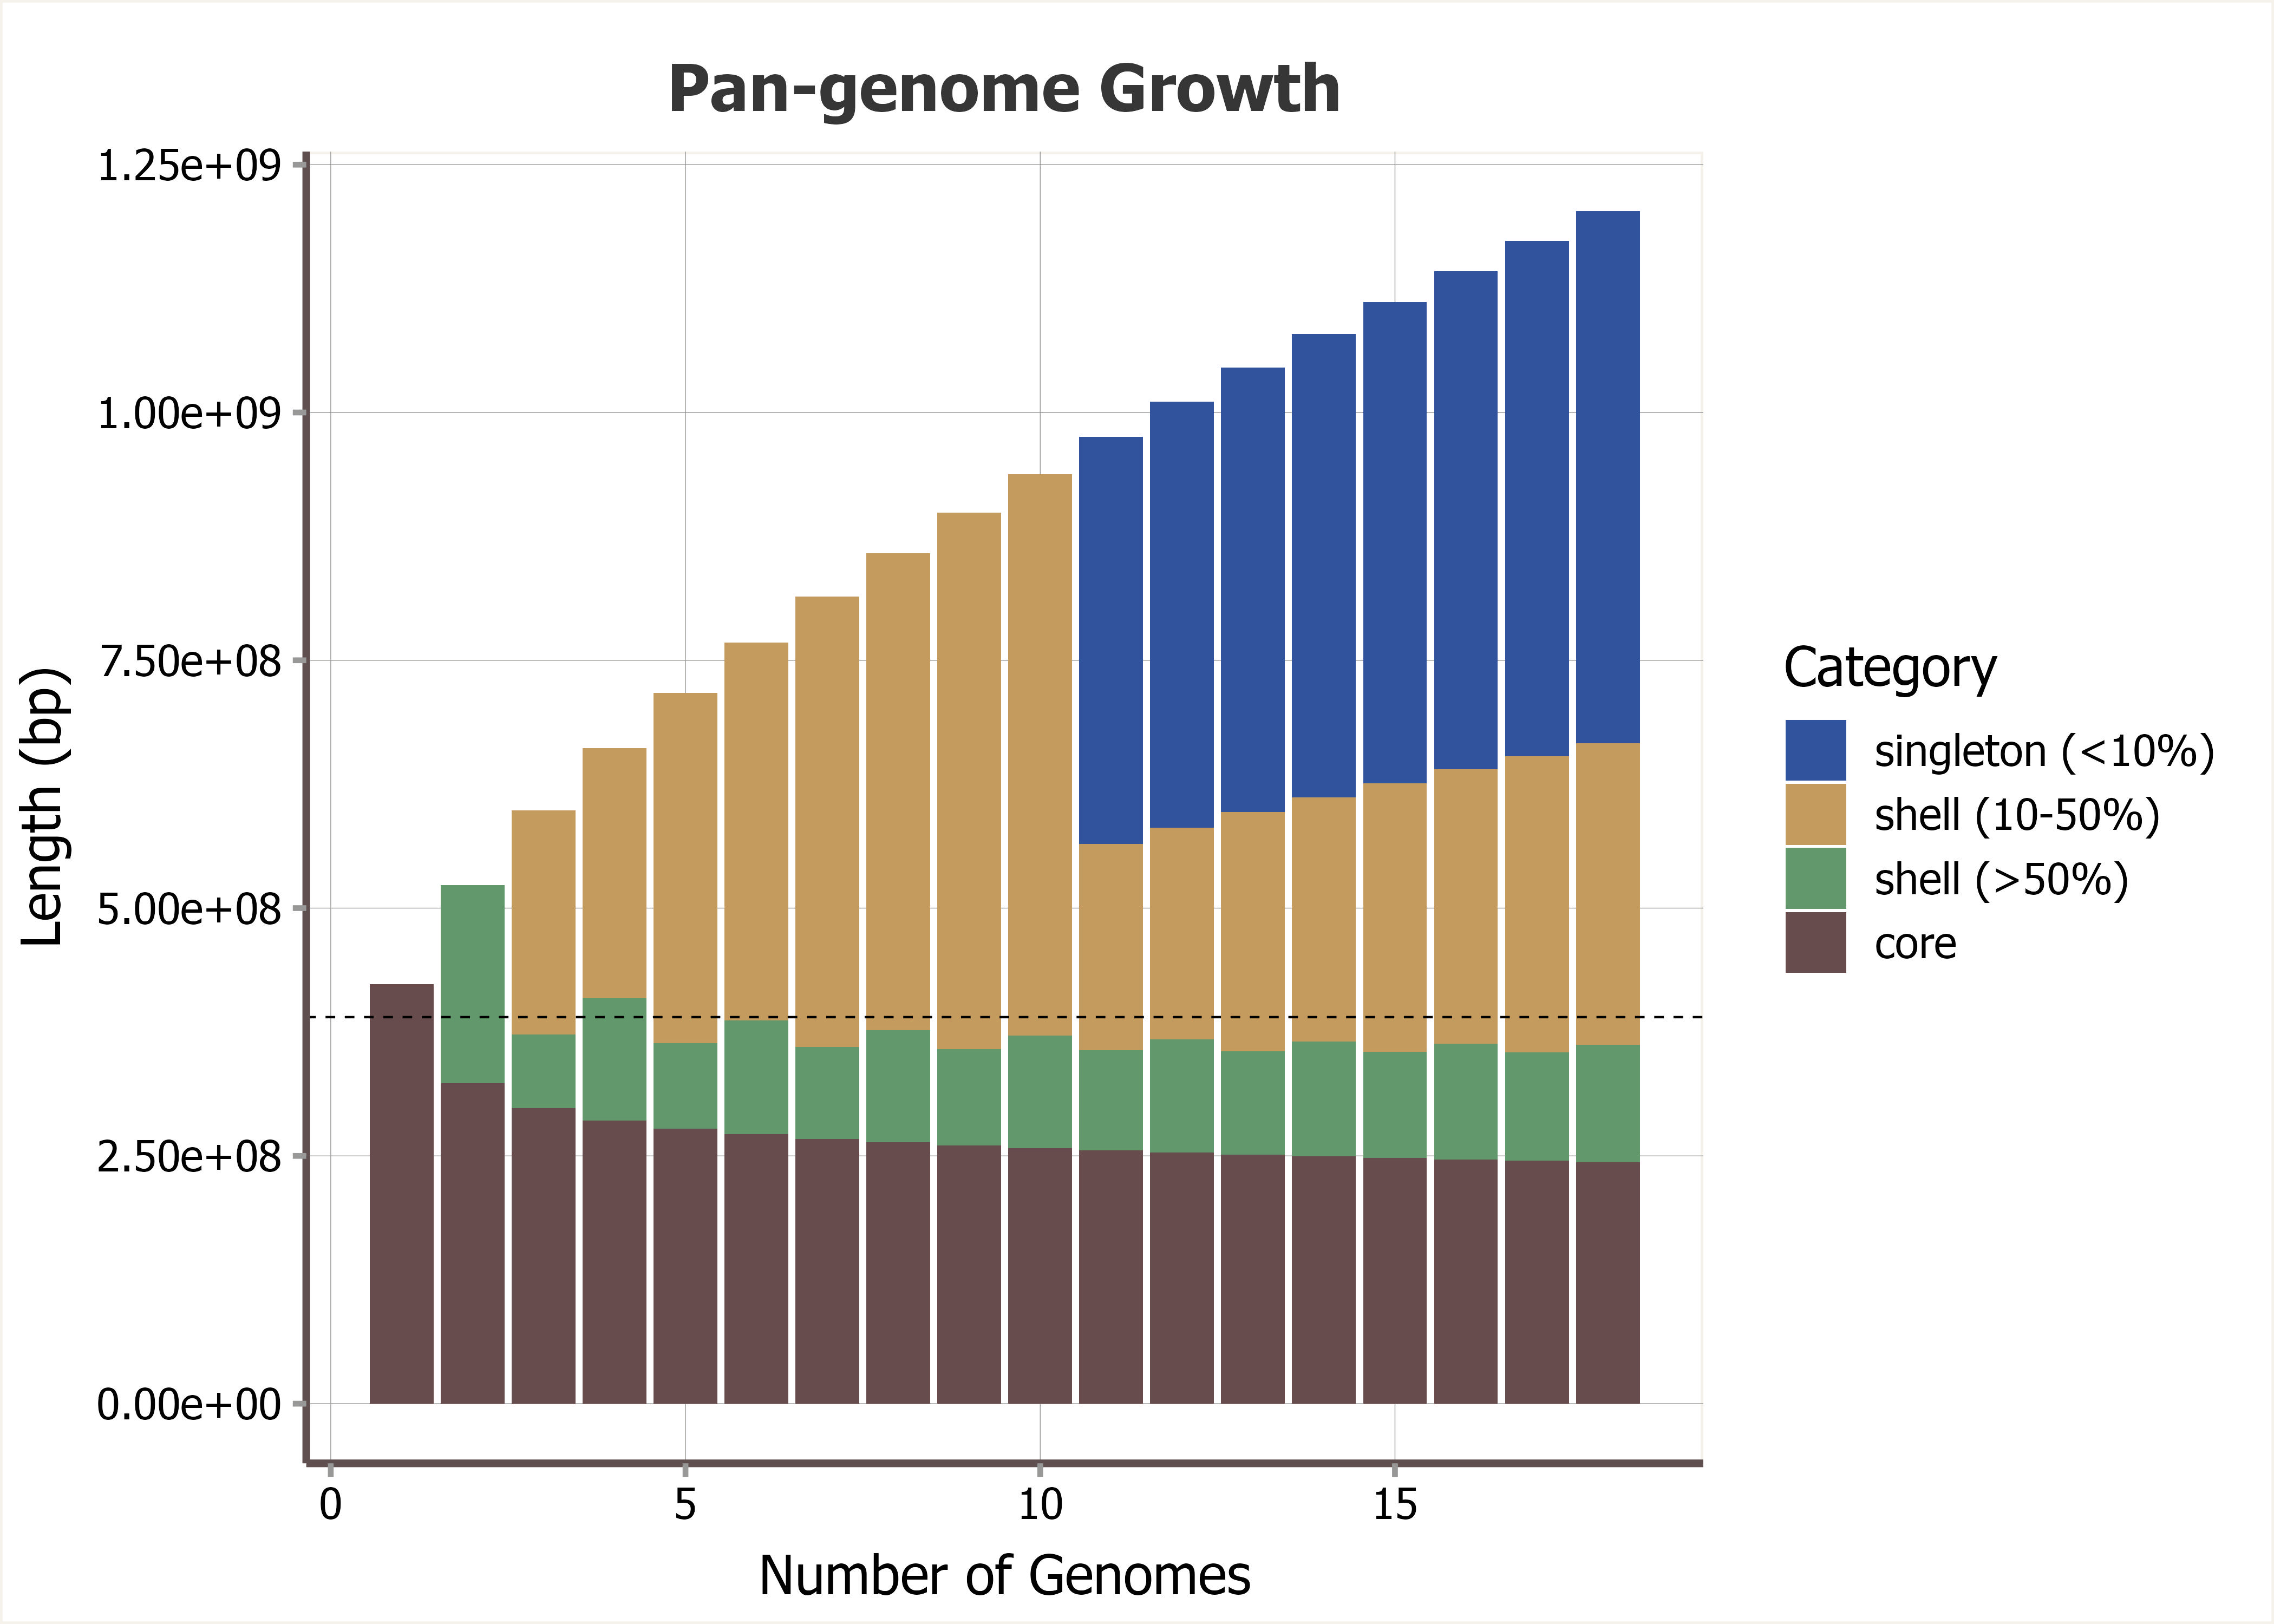
\includegraphics[keepaspectratio]{figs/pg_growth.jpg}}

}

\subcaption{\label{fig-2a}}

\end{minipage}%
%
\begin{minipage}{0.50\linewidth}

\centering{

\pandocbounded{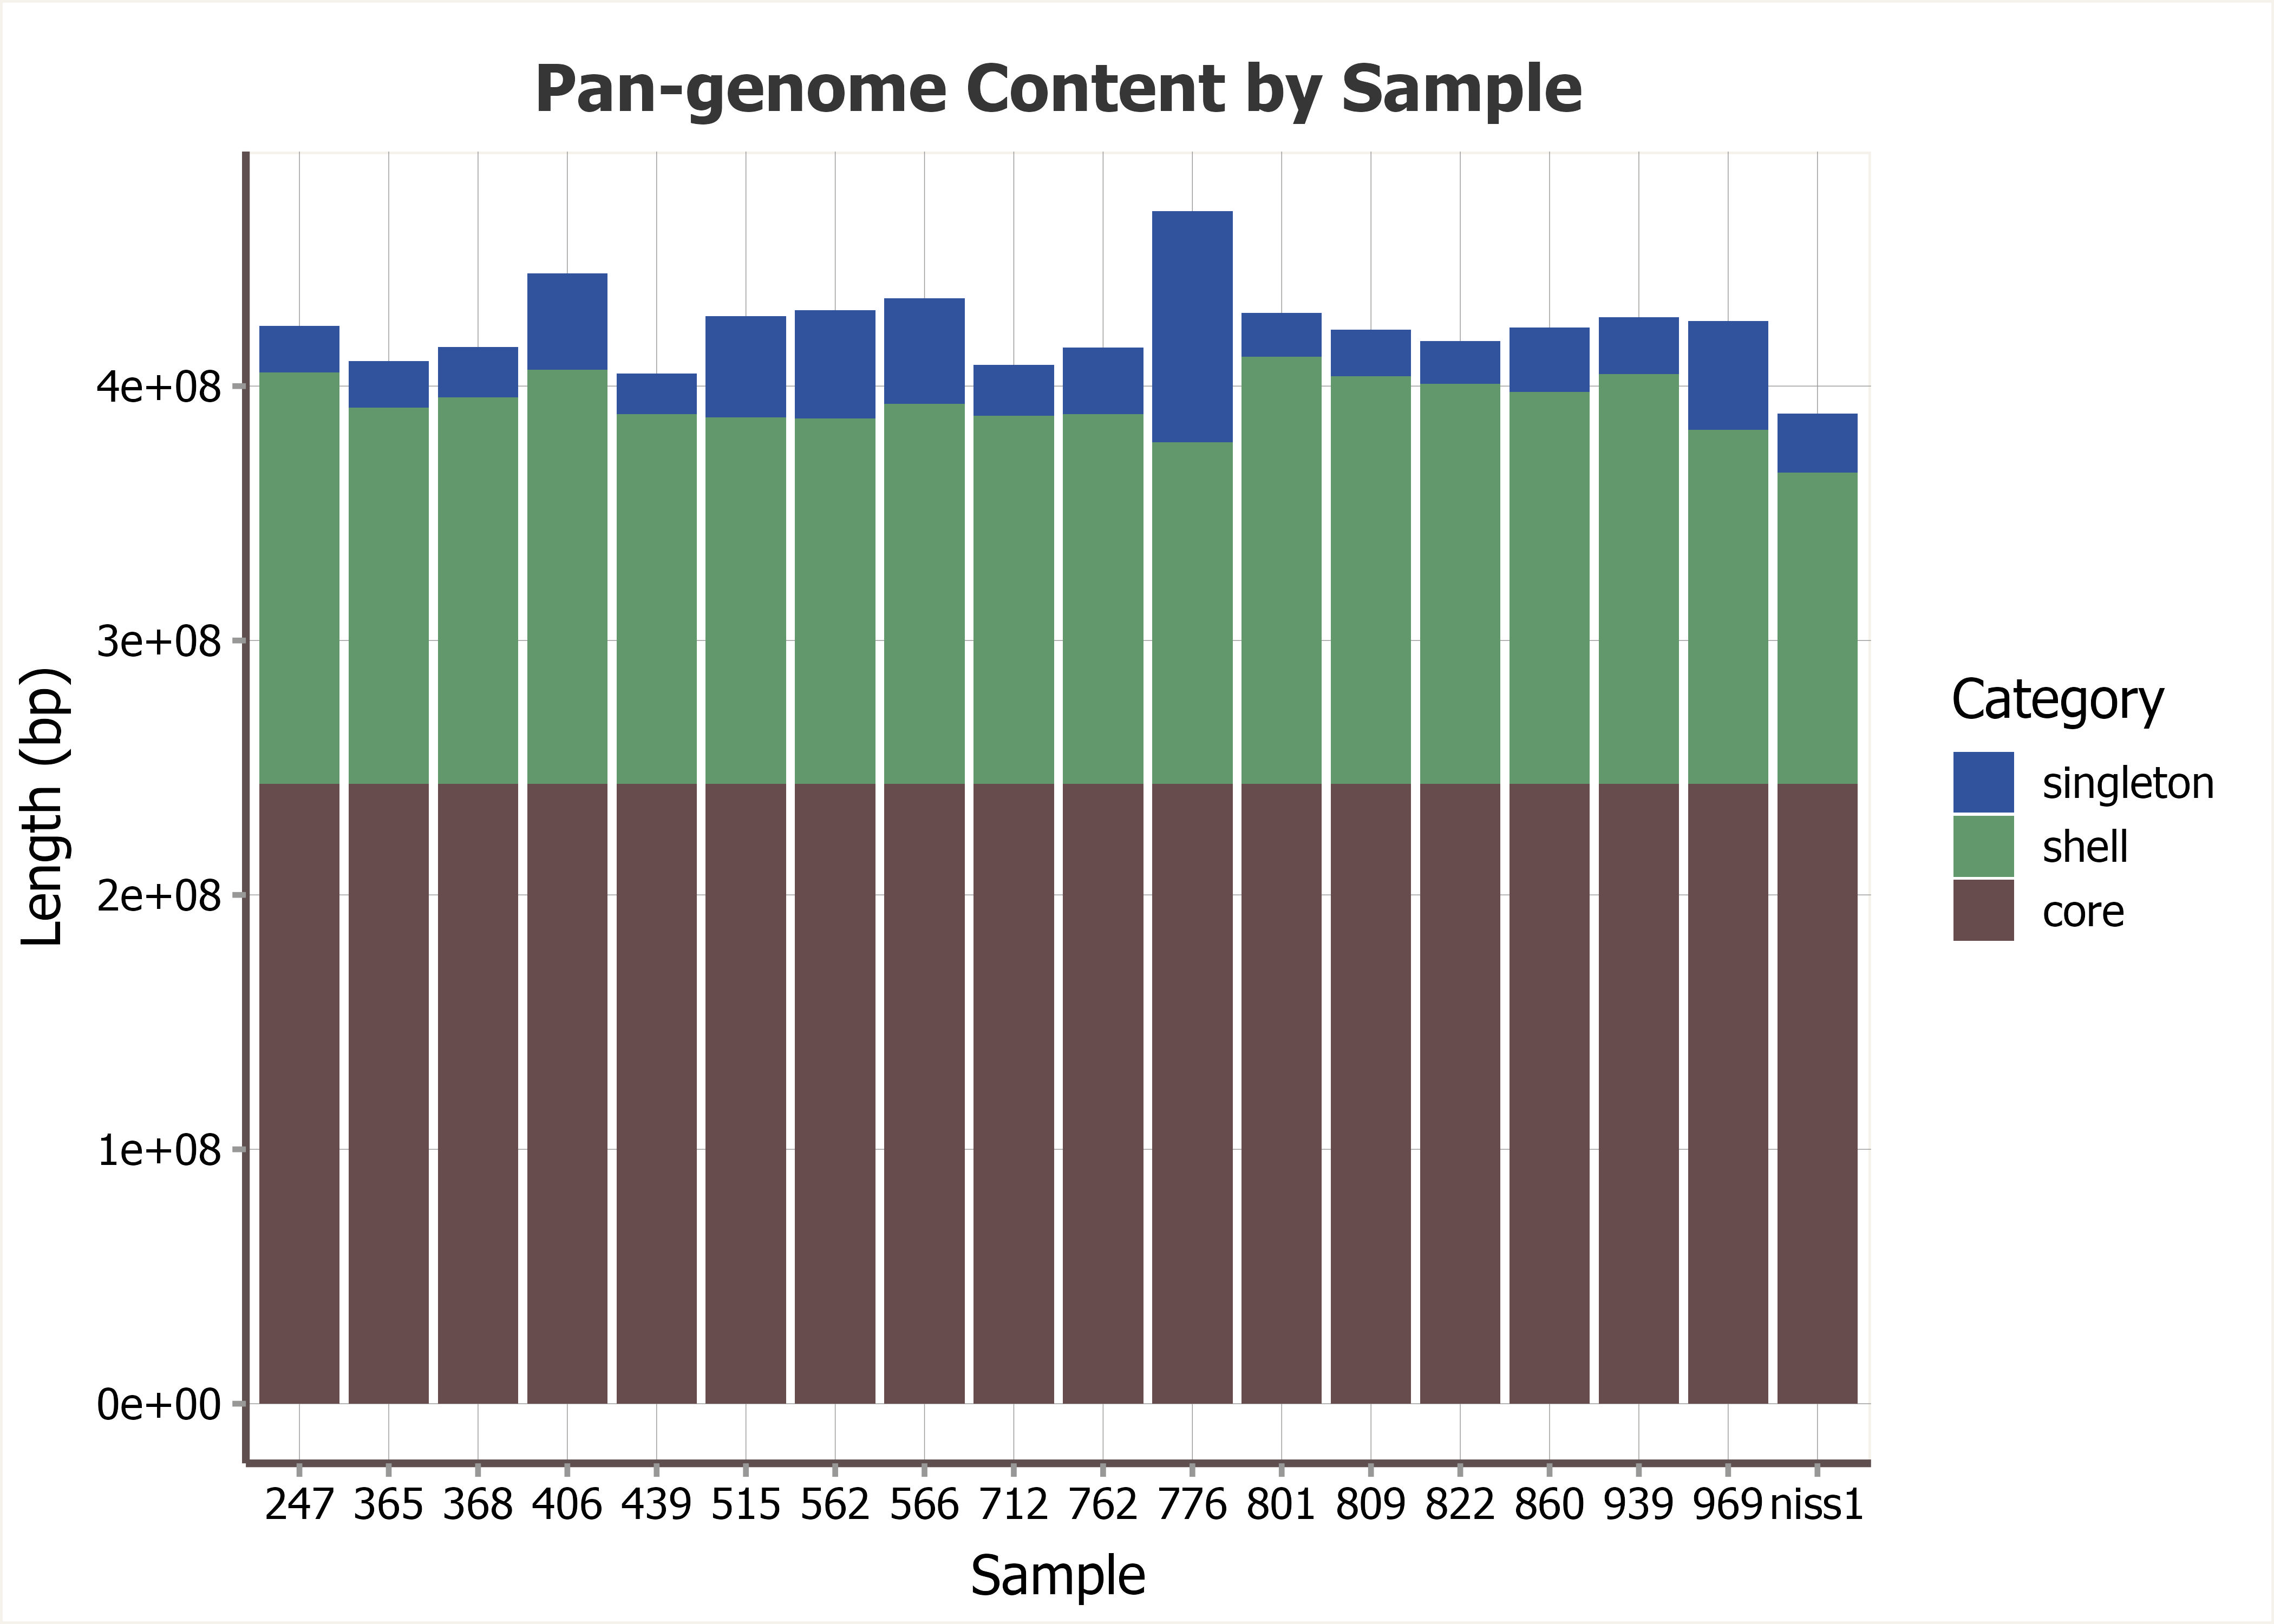
\includegraphics[keepaspectratio]{figs/pg_content.jpg}}

}

\subcaption{\label{fig-2b}}

\end{minipage}%

\caption{\label{fig-2}(a): Pan-genome growth curve visualizes the change
in core and shell genome size as samples are added. (b): The relative
length of the core, shell and singleton portions of the pan-genome for
each sample represented}

\end{figure}%

\begin{figure}

\begin{minipage}{0.33\linewidth}
\pandocbounded{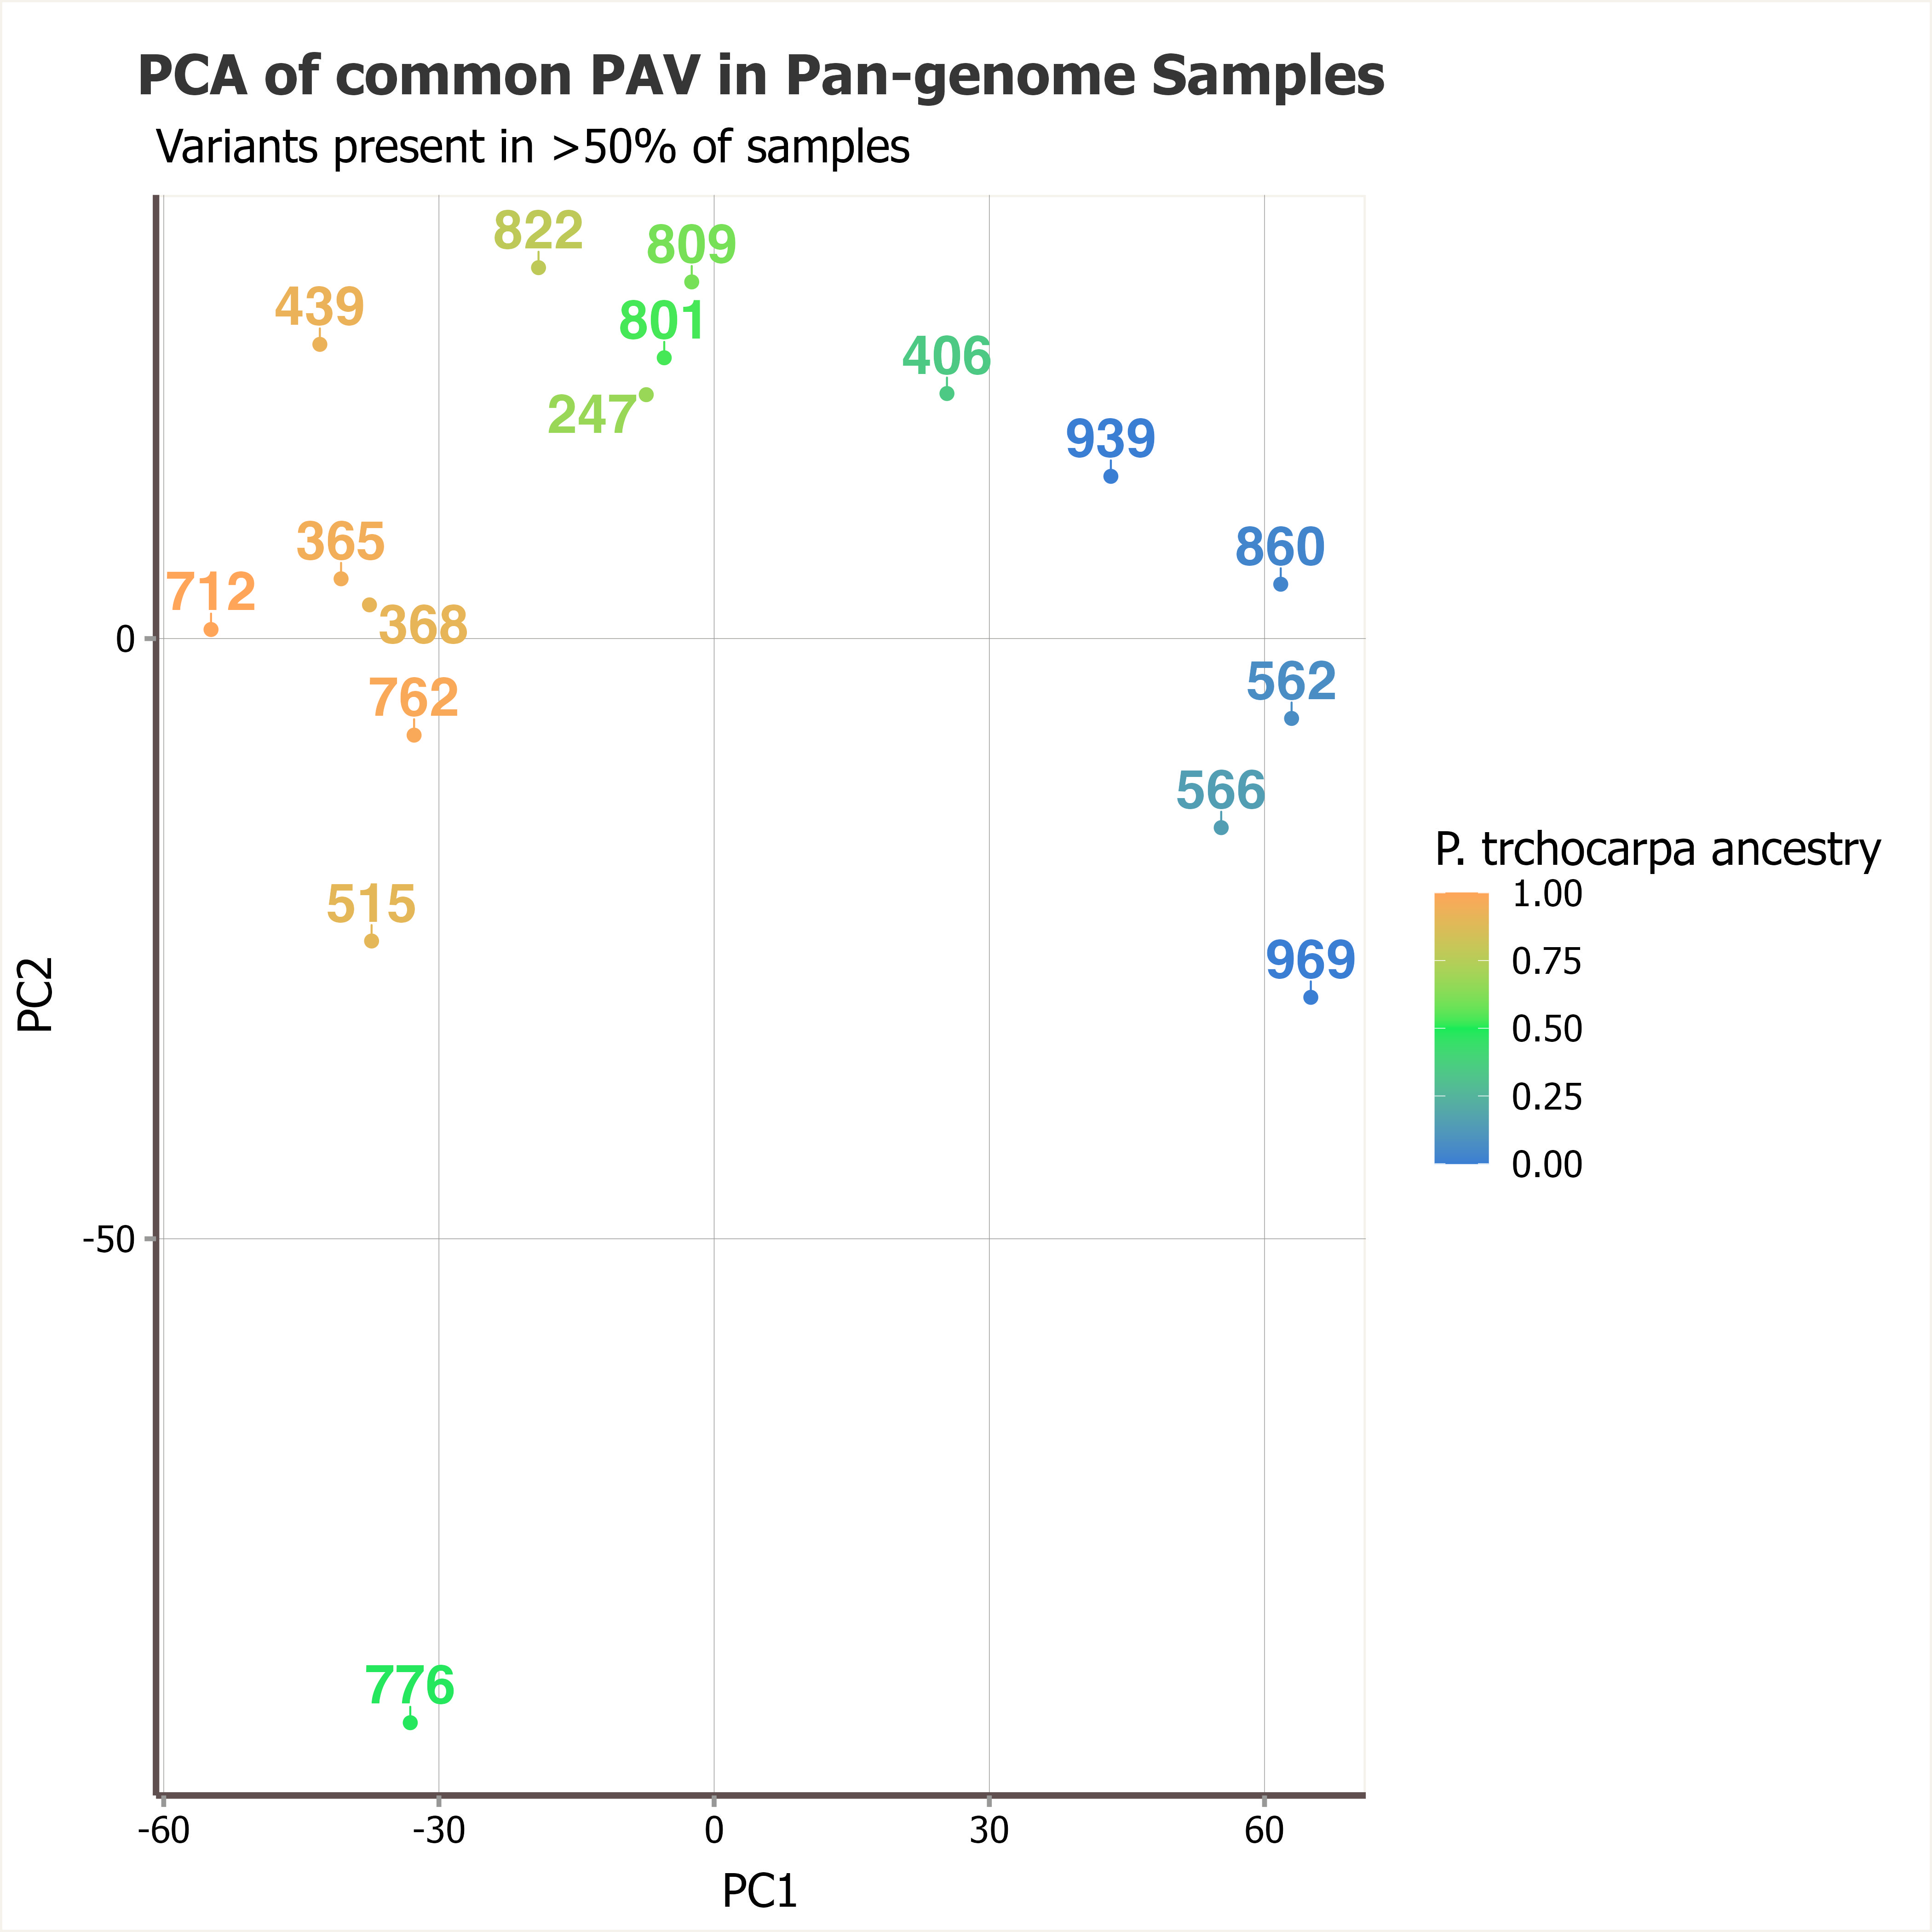
\includegraphics[keepaspectratio]{figs/com_pav_pca.jpg}}
\pandocbounded{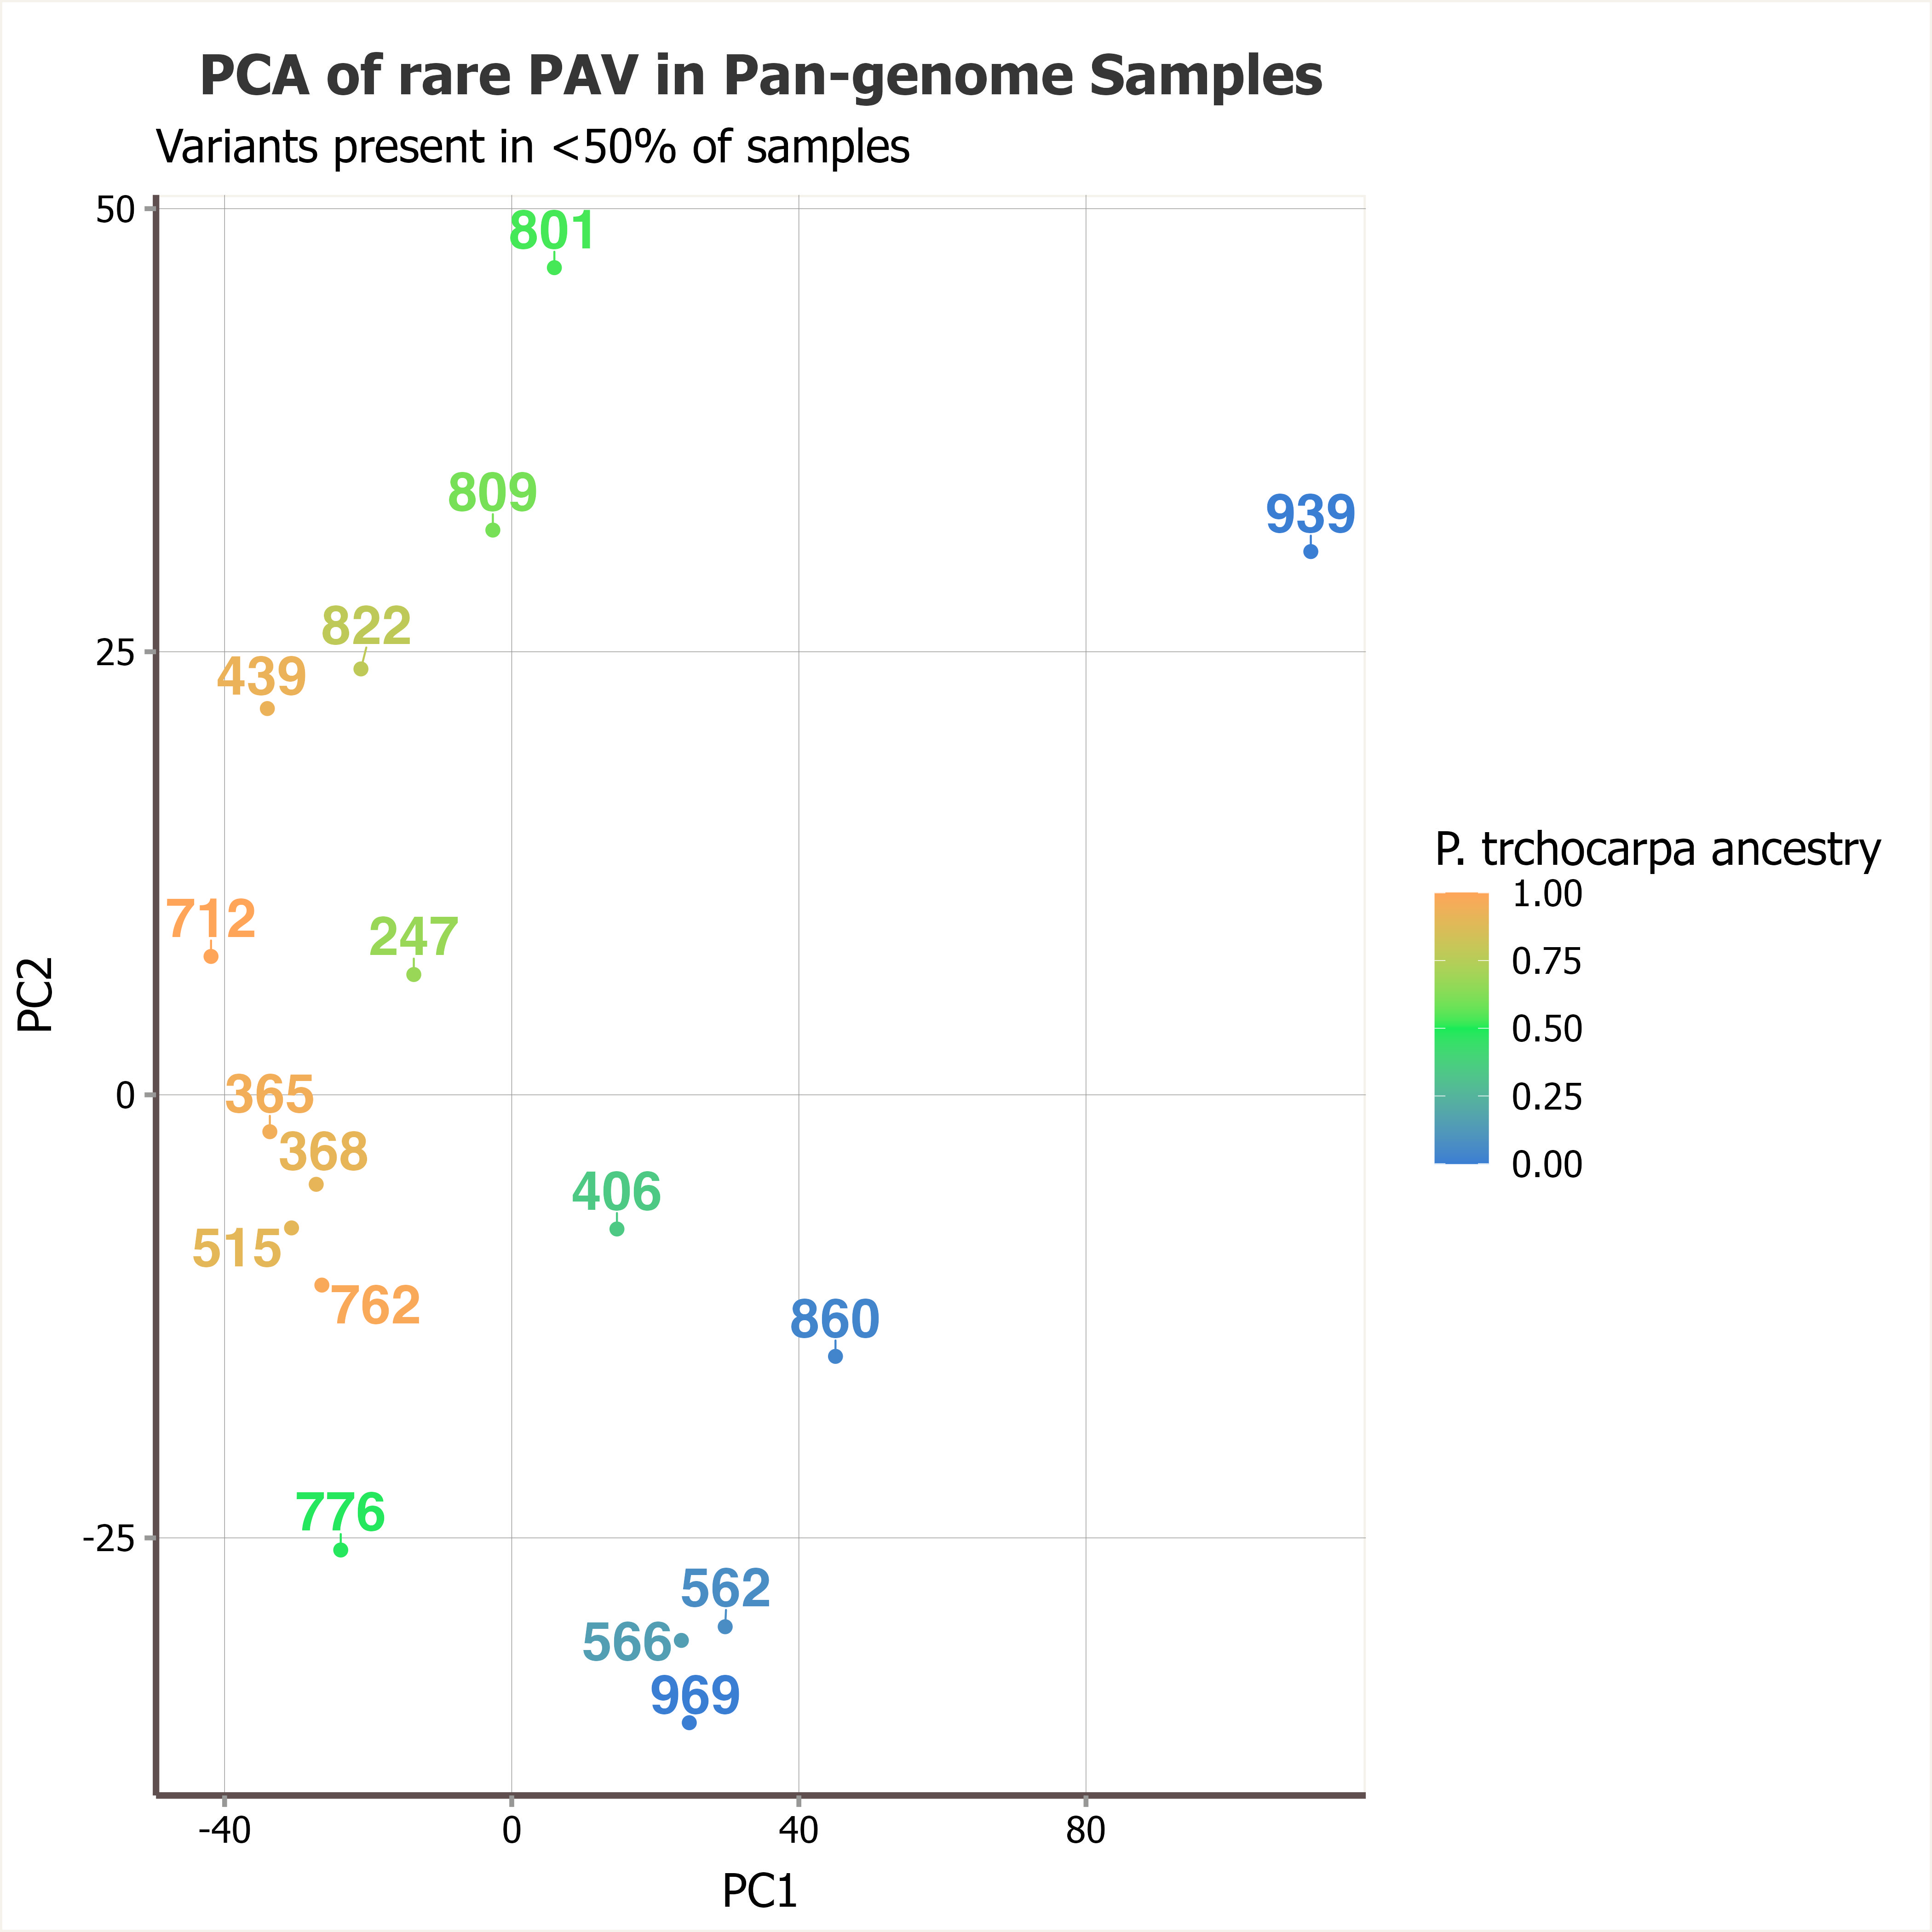
\includegraphics[keepaspectratio]{figs/rar_pav_pca.jpg}}\end{minipage}%
%
\begin{minipage}{0.33\linewidth}

\centering{

\pandocbounded{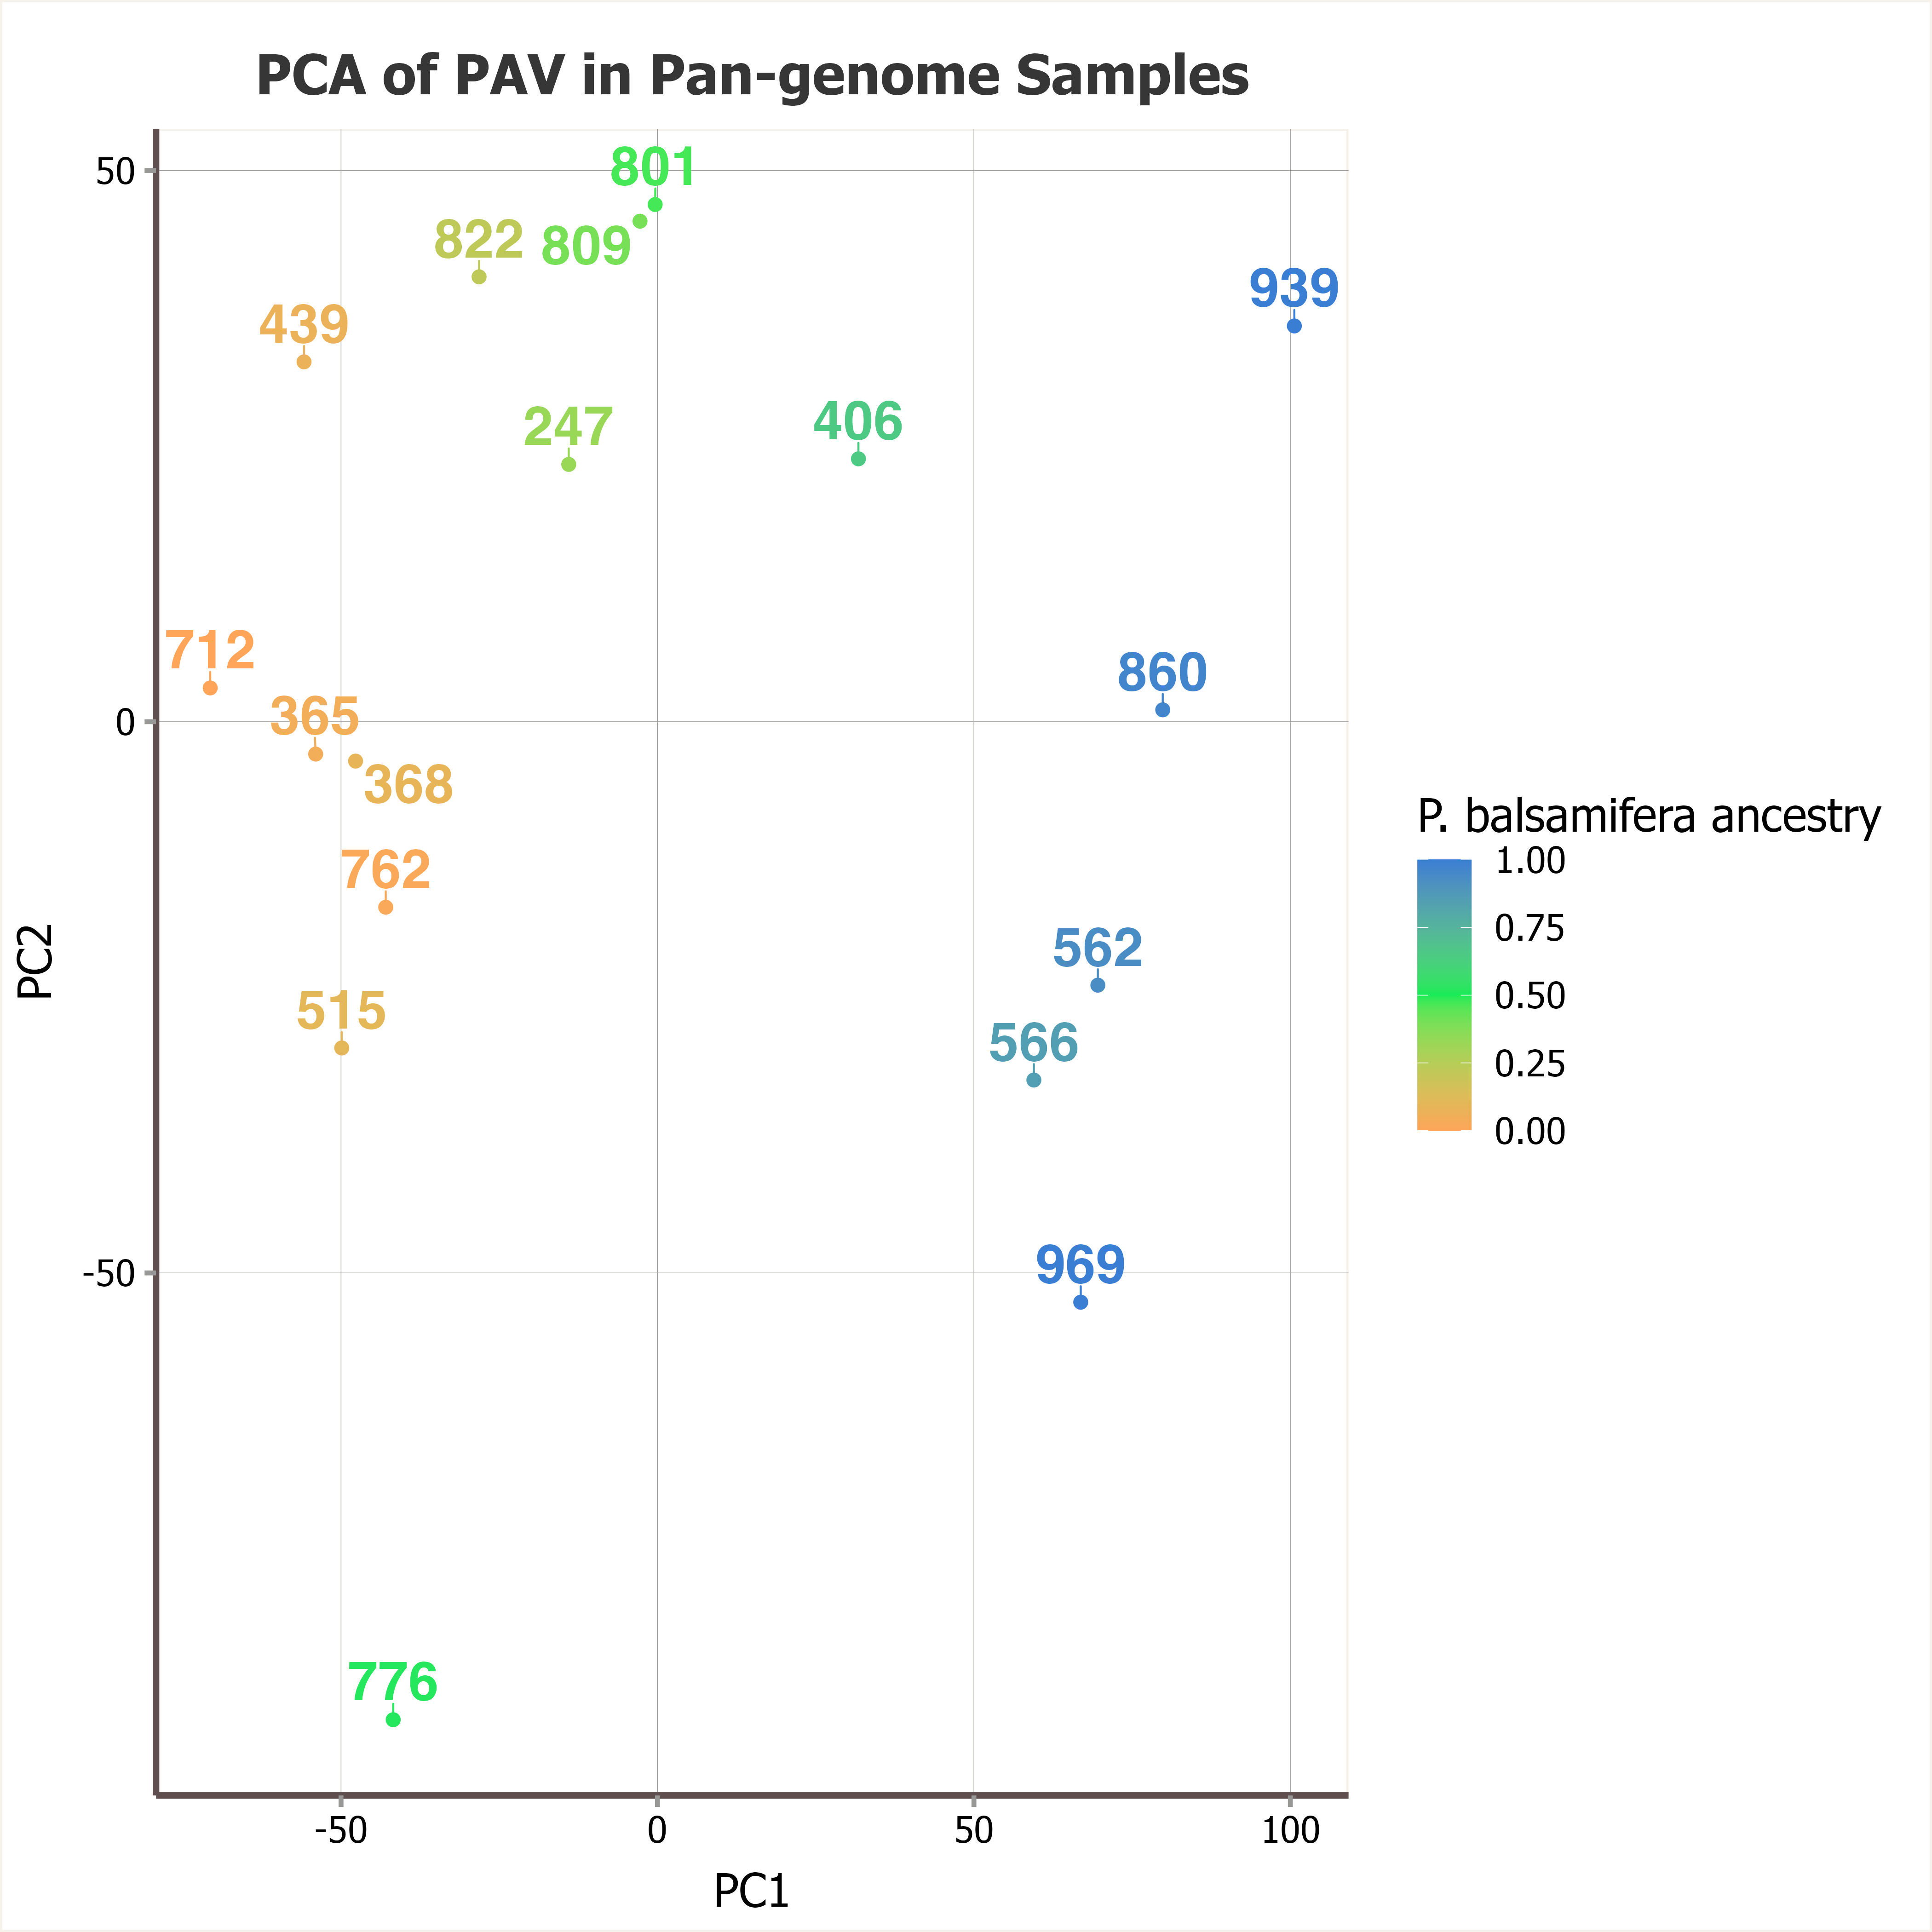
\includegraphics[keepaspectratio]{figs/pav_pca.jpg}}

}

\subcaption{\label{fig-3c}}

\end{minipage}%

\caption{\label{fig-3}The first two principal components of a PCA on
presence/absence variation in the pan-genome. Results of PCA on common
(a), rare (b) and all (c) PAV are shown Color indicates ancestry based
in ADMIXTURE analysis.}

\end{figure}%

\begin{figure}

\centering{

\pandocbounded{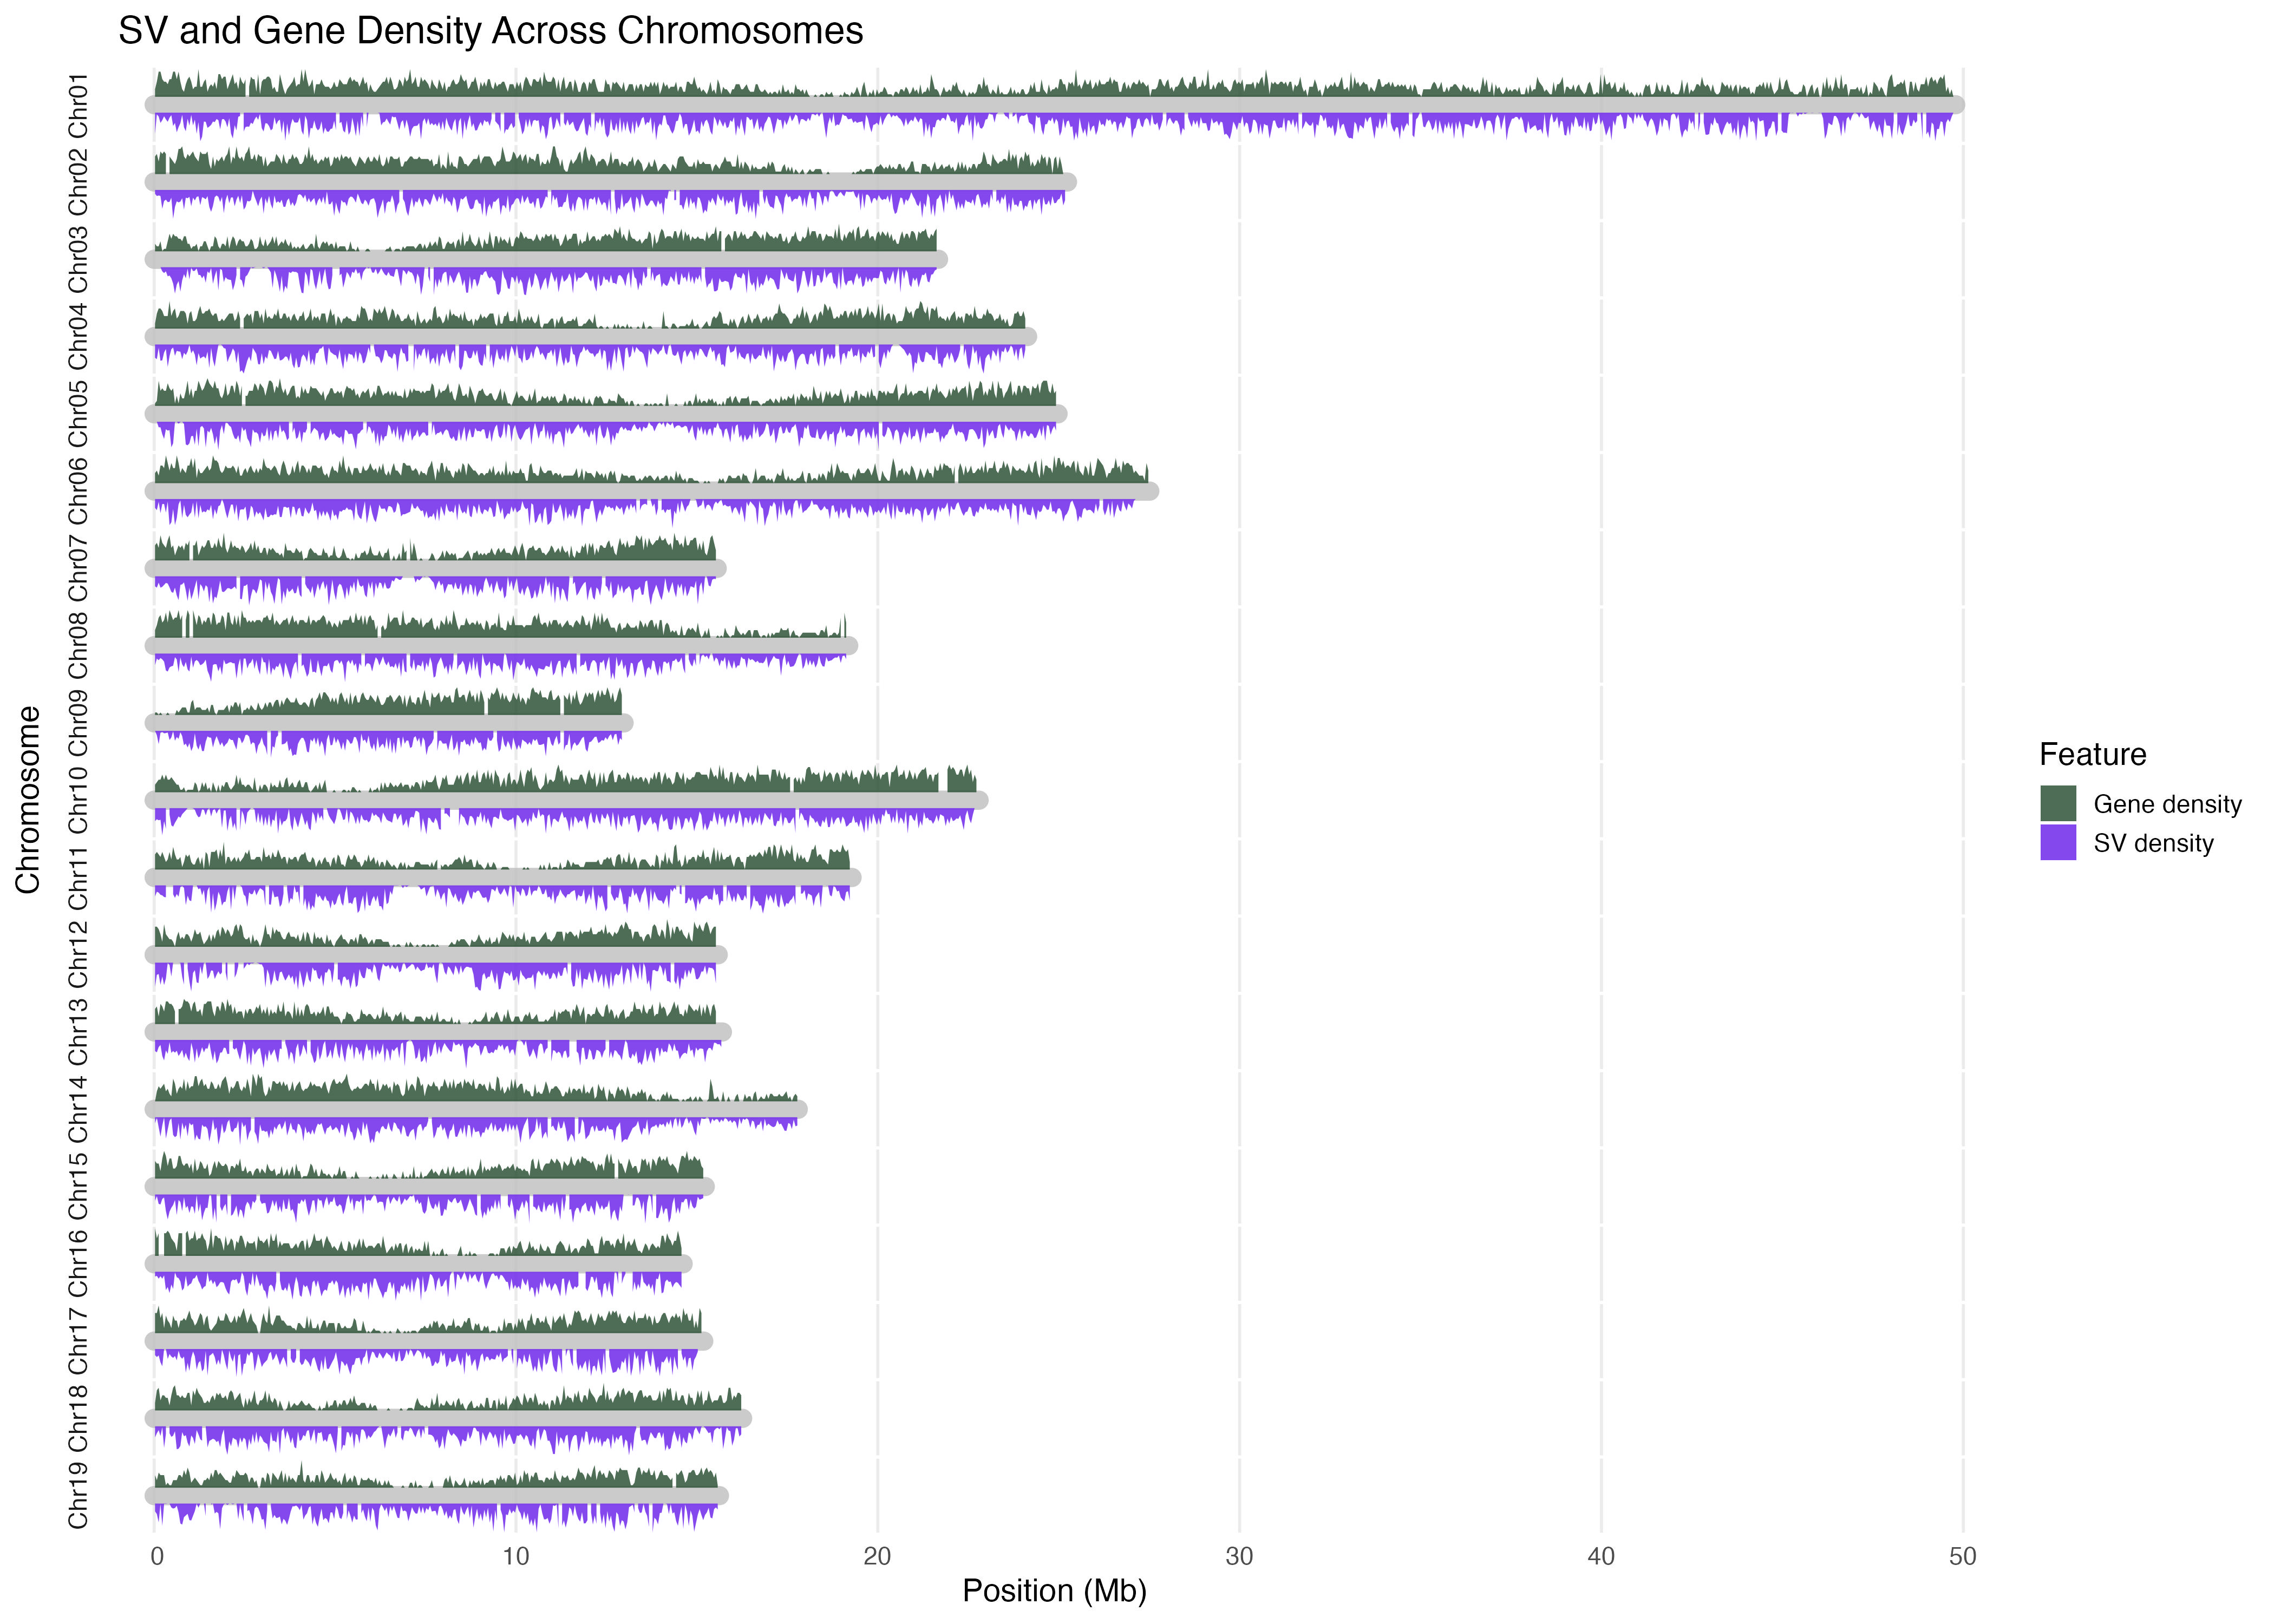
\includegraphics[keepaspectratio]{figs/sv_genomic_distribution.jpg}}

}

\caption{\label{fig-5}The density of SV larger than 20bp in length
across the genome (purple) compared to the density of annotated genes
(green)}

\end{figure}%

\begin{figure}

\centering{

\pandocbounded{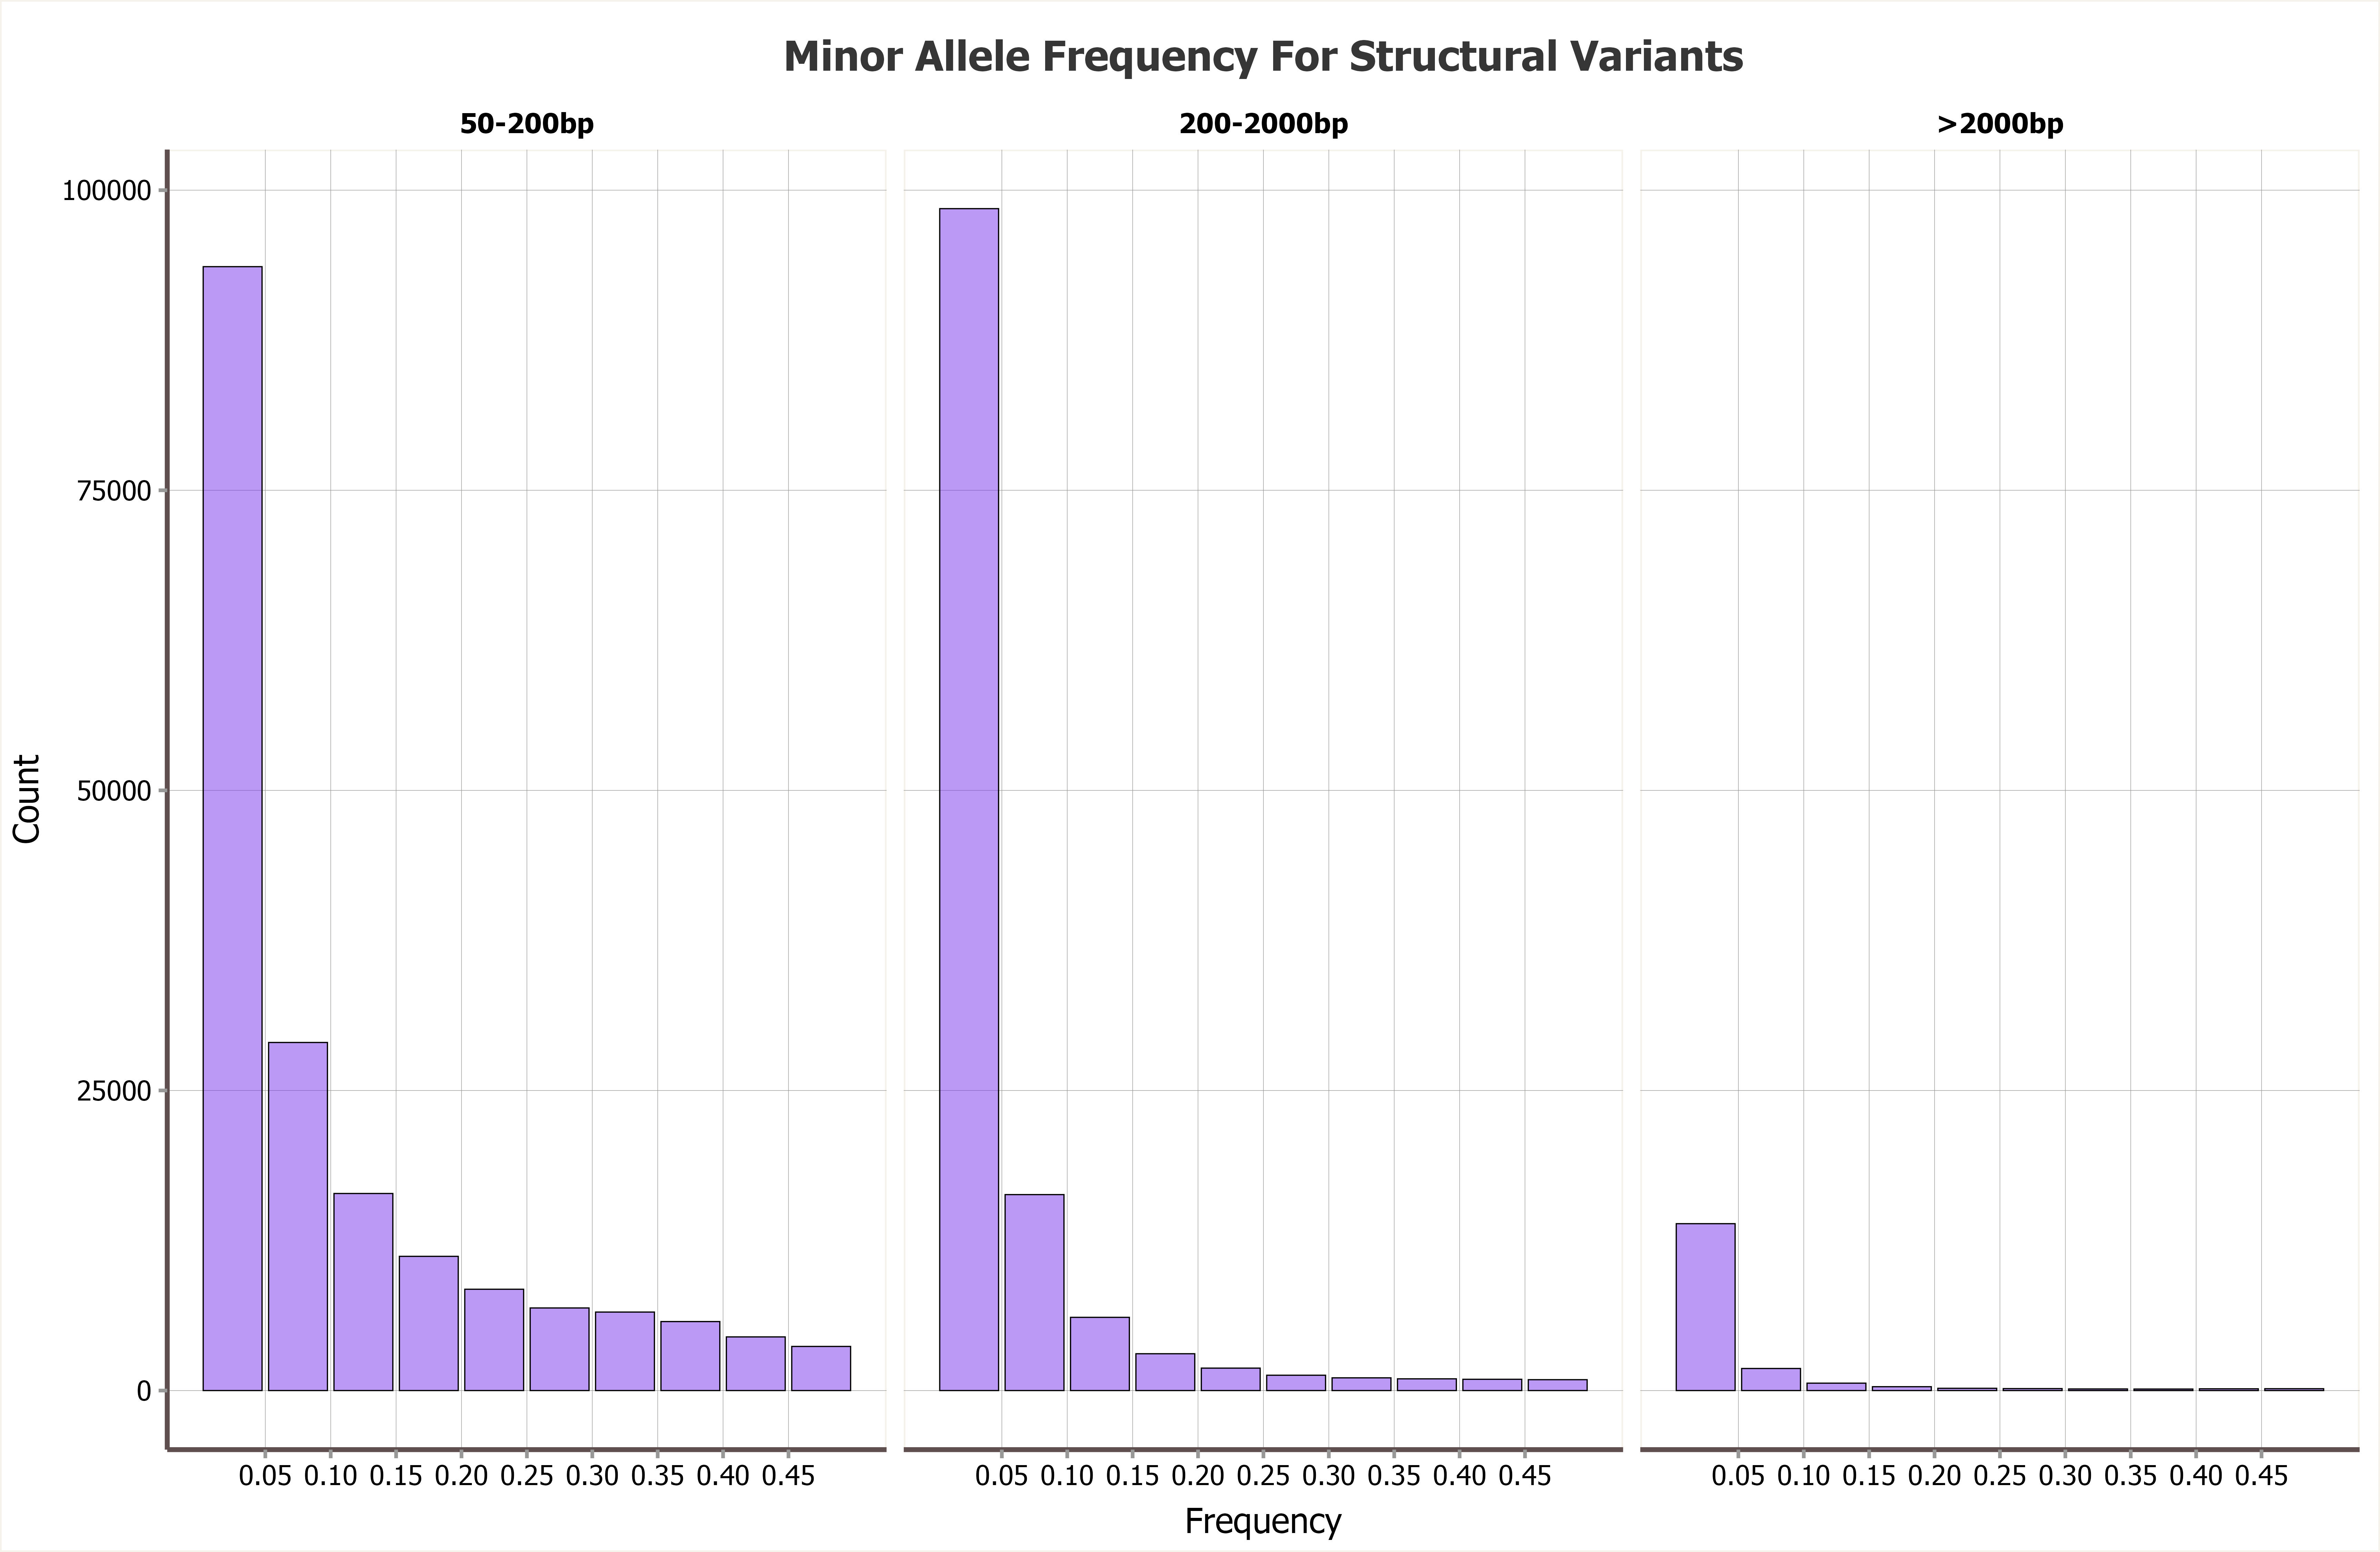
\includegraphics[keepaspectratio]{figs/sv_freq.jpg}}

}

\caption{\label{fig-6}The frequency distribution of the minor allele for
SV of different size classes}

\end{figure}%

\begin{figure}

\centering{

\pandocbounded{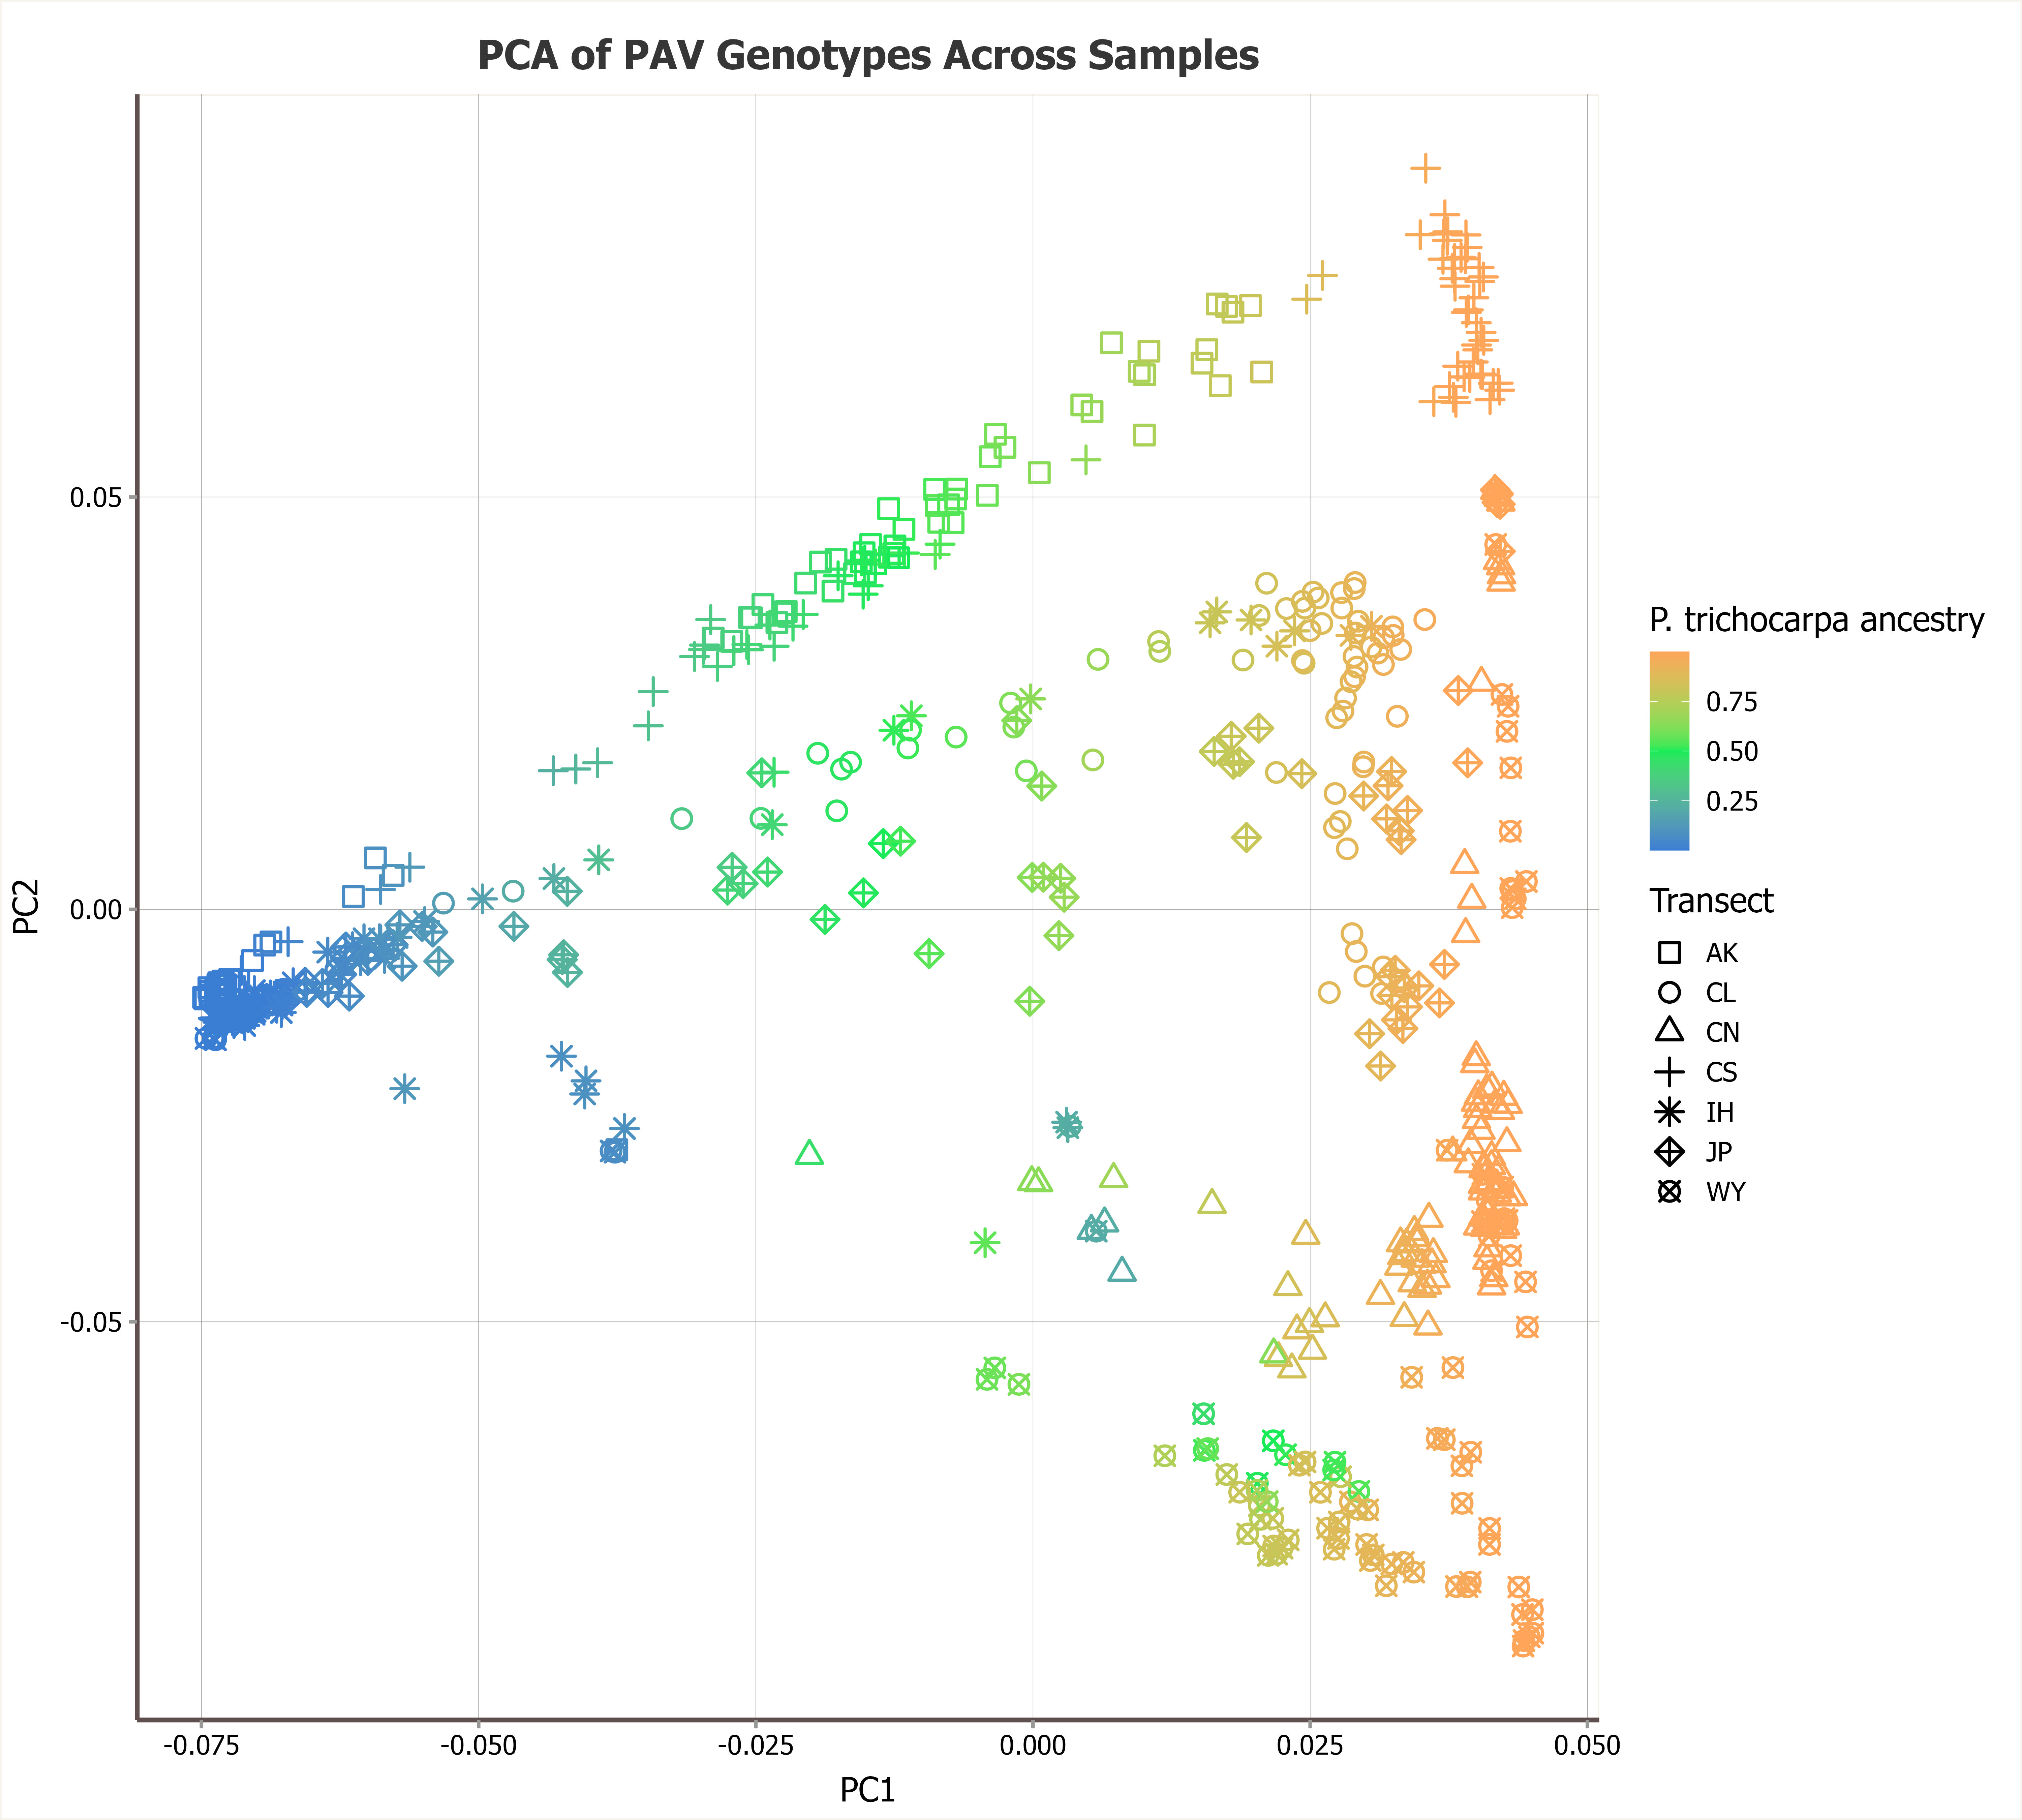
\includegraphics[keepaspectratio]{figs/sv_pc1_pc2.jpg}}

}

\caption{\label{fig-7}The first two principal components of a PCA of PAV
genotyped from short read alignments to the pan-genome graph. Color
indicates ancestry based on ADMIXTURE analysis. Shape indicates which of
the latitudinal transects the individual was sampled from.}

\end{figure}%

\subsection*{References}\label{references}
\addcontentsline{toc}{subsection}{References}

\phantomsection\label{refs}
\begin{CSLReferences}{1}{0}
\vspace{1em}

\bibitem[\citeproctext]{ref-almarri2020population}
Almarri, M. A., Bergström, A., Prado-Martinez, J., Yang, F., Fu, B.,
Dunham, A. S., et al. (2020). Population structure, stratification, and
introgression of human structural variation. \emph{Cell}, \emph{182}(1),
189--199.

\bibitem[\citeproctext]{ref-bock2023genomics}
Bock, D. G., Cai, Z., Elphinstone, C., Gonzalez-Segovia, E.,
Hirabayashi, K., Huang, K., et al. (2023). Genomics of plant speciation.
\emph{Plant Communications}, \emph{4}(5).

\bibitem[\citeproctext]{ref-burgarella2019adaptive}
Burgarella, C., Barnaud, A., Kane, N. A., Jankowski, F., Scarcelli, N.,
Billot, C., et al. (2019). Adaptive introgression: An untapped
evolutionary mechanism for crop adaptation. \emph{Frontiers in Plant
Science}, \emph{10}, 4.

\bibitem[\citeproctext]{ref-chang2015second}
Chang, C. C., Chow, C. C., Tellier, L. C., Vattikuti, S., Purcell, S.
M., \& Lee, J. J. (2015). Second-generation PLINK: Rising to the
challenge of larger and richer datasets. \emph{Gigascience},
\emph{4}(1), s13742--015.

\bibitem[\citeproctext]{ref-cheng2019frequent}
Cheng, H., Liu, J., Wen, J., Nie, X., Xu, L., Chen, N., et al. (2019).
Frequent intra-and inter-species introgression shapes the landscape of
genetic variation in bread wheat. \emph{Genome Biology}, \emph{20},
1--16.

\bibitem[\citeproctext]{ref-chhatre2018adaptive}
Chhatre, V. E., Evans, L. M., DiFazio, S. P., \& Keller, S. R. (2018).
Adaptive introgression and maintenance of a trispecies hybrid complex in
range-edge populations of populus. \emph{Molecular Ecology},
\emph{27}(23), 4820--4838.

\bibitem[\citeproctext]{ref-danecek2021}
Danecek, P., Bonfield, J. K., Liddle, J., Marshall, J., Ohan, V.,
Pollard, M. O., et al. (2021). Twelve years of SAMtools and BCFtools.
\emph{GigaScience}, \emph{10}(2).
\url{https://doi.org/10.1093/gigascience/giab008}

\bibitem[\citeproctext]{ref-dias2018loter}
Dias-Alves, T., Mairal, J., \& Blum, M. G. (2018). Loter: A software
package to infer local ancestry for a wide range of species.
\emph{Molecular Biology and Evolution}, \emph{35}(9), 2318--2326.

\bibitem[\citeproctext]{ref-fang2024fitness}
Fang, B., \& Edwards, S. V. (2024). Fitness consequences of structural
variation inferred from a house finch pangenome. \emph{Proceedings of
the National Academy of Sciences}, \emph{121}(47), e2409943121.

\bibitem[\citeproctext]{ref-feng2024integrating}
Feng, J., Dan, X., Cui, Y., Gong, Y., Peng, M., Sang, Y., et al. (2024).
Integrating evolutionary genomics of forest trees to inform future tree
breeding amid rapid climate change. \emph{Plant Communications},
\emph{5}(10).

\bibitem[\citeproctext]{ref-ferguson2024exploring}
Ferguson, S., Jones, A., Murray, K., Andrew, R. L., Schwessinger, B.,
Bothwell, H., \& Borevitz, J. (2024). Exploring the role of polymorphic
interspecies structural variants in reproductive isolation and adaptive
divergence in eucalyptus. \emph{GigaScience}, \emph{13}, giae029.

\bibitem[\citeproctext]{ref-fetter2023admixture}
Fetter, K. C., \& Keller, S. R. (2023). Admixture mapping and selection
scans identify genomic regions associated with stomatal patterning and
disease resistance in hybrid poplars. \emph{Ecology and Evolution},
\emph{13}(10), e10579.

\bibitem[\citeproctext]{ref-gaczorek2024widespread}
Gaczorek, T., Dudek, K., Fritz, U., Bahri-Sfar, L., Baird, S., Bonhomme,
F., et al. (2024). Widespread adaptive introgression of major
histocompatibility complex genes across vertebrate hybrid zones.
\emph{Molecular Biology and Evolution}, \emph{41}(10), msae201.

\bibitem[\citeproctext]{ref-gao2019tomato}
Gao, L., Gonda, I., Sun, H., Ma, Q., Bao, K., Tieman, D. M., et al.
(2019). The tomato pan-genome uncovers new genes and a rare allele
regulating fruit flavor. \emph{Nature Genetics}, \emph{51}(6),
1044--1051.

\bibitem[\citeproctext]{ref-garrison2018}
Garrison, E., Sirén, J., Novak, A. M., Hickey, G., Eizenga, J. M.,
Dawson, E. T., et al. (2018). Variation graph toolkit improves read
mapping by representing genetic variation in the reference. \emph{Nature
Biotechnology}, \emph{36}(9), 875--879.
\url{https://doi.org/10.1038/nbt.4227}

\bibitem[\citeproctext]{ref-geraldes2014landscape}
Geraldes, A., Farzaneh, N., Grassa, C. J., McKown, A. D., Guy, R. D.,
Mansfield, S. D., et al. (2014). Landscape genomics of populus
trichocarpa: The role of hybridization, limited gene flow, and natural
selection in shaping patterns of population structure. \emph{Evolution},
\emph{68}(11), 3260--3280.

\bibitem[\citeproctext]{ref-gurevich2013quast}
Gurevich, A., Saveliev, V., Vyahhi, N., \& Tesler, G. (2013). QUAST:
Quality assessment tool for genome assemblies. \emph{Bioinformatics},
\emph{29}(8), 1072--1075.

\bibitem[\citeproctext]{ref-hamala2021genomic}
Hämälä, T., Wafula, E. K., Guiltinan, M. J., Ralph, P. E., Depamphilis,
C. W., \& Tiffin, P. (2021). Genomic structural variants constrain and
facilitate adaptation in natural populations of theobroma cacao, the
chocolate tree. \emph{Proceedings of the National Academy of Sciences},
\emph{118}(35), e2102914118.

\bibitem[\citeproctext]{ref-hamilton2016adaptive}
Hamilton, J. A., \& Miller, J. M. (2016). Adaptive introgression as a
resource for management and genetic conservation in a changing climate.
\emph{Conservation Biology}, \emph{30}(1), 33--41.

\bibitem[\citeproctext]{ref-hedrick2013adaptive}
Hedrick, P. W. (2013). Adaptive introgression in animals: Examples and
comparison to new mutation and standing variation as sources of adaptive
variation. \emph{Molecular Ecology}, \emph{22}(18), 4606--4618.

\bibitem[\citeproctext]{ref-hickey2023}
Hickey, G., Monlong, J., Ebler, J., Novak, A. M., Eizenga, J. M., Gao,
Y., et al. (2023). Pangenome graph construction from genome alignments
with Minigraph-Cactus. \emph{Nature Biotechnology}, \emph{42}(4),
663--673. \url{https://doi.org/10.1038/s41587-023-01793-w}

\bibitem[\citeproctext]{ref-kang2023pan}
Kang, M., Wu, H., Liu, H., Liu, W., Zhu, M., Han, Y., et al. (2023). The
pan-genome and local adaptation of arabidopsis thaliana. \emph{Nature
Communications}, \emph{14}(1), 6259.

\bibitem[\citeproctext]{ref-kou2020evolutionary}
Kou, Y., Liao, Y., Toivainen, T., Lv, Y., Tian, X., Emerson, J., et al.
(2020). Evolutionary genomics of structural variation in asian rice
(oryza sativa) domestication. \emph{Molecular Biology and Evolution},
\emph{37}(12), 3507--3524.

\bibitem[\citeproctext]{ref-kremer2020oaks}
Kremer, A., \& Hipp, A. L. (2020). Oaks: An evolutionary success story.
\emph{New Phytologist}, \emph{226}(4), 987--1011.

\bibitem[\citeproctext]{ref-leroy2020adaptive}
Leroy, T., Louvet, J.-M., Lalanne, C., Le Provost, G., Labadie, K.,
Aury, J.-M., et al. (2020). Adaptive introgression as a driver of local
adaptation to climate in european white oaks. \emph{New Phytologist},
\emph{226}(4), 1171--1182.

\bibitem[\citeproctext]{ref-lexer2005barrier}
Lexer, C., Fay, M., Joseph, J., Nica, M.-S., \& Heinze, B. (2005).
Barrier to gene flow between two ecologically divergent populus species,
p. Alba (white poplar) and p. Tremula (european aspen): The role of
ecology and life history in gene introgression. \emph{Molecular
Ecology}, \emph{14}(4), 1045--1057.

\bibitem[\citeproctext]{ref-li2018minimap2}
Li, H. (2018). Minimap2: Pairwise alignment for nucleotide sequences.
\emph{Bioinformatics}, \emph{34}(18), 3094--3100.

\bibitem[\citeproctext]{ref-li2010fast}
Li, H., \& Durbin, R. (2010). Fast and accurate long-read alignment with
burrows--wheeler transform. \emph{Bioinformatics}, \emph{26}(5),
589--595.

\bibitem[\citeproctext]{ref-li2023identification}
Li, K., Xu, P., Wang, J., Yi, X., \& Jiao, Y. (2023). Identification of
errors in draft genome assemblies at single-nucleotide resolution for
quality assessment and improvement. \emph{Nature Communications},
\emph{14}(1), 6556.

\bibitem[\citeproctext]{ref-li2024pan}
Li, Y., Yao, J., Sang, H., Wang, Q., Su, L., Zhao, X., et al. (2024).
Pan-genome analysis highlights the role of structural variation in the
evolution and environmental adaptation of asian honeybees.
\emph{Molecular Ecology Resources}, \emph{24}(2), e13905.

\bibitem[\citeproctext]{ref-li2023pig}
Li, Z., Liu, X., Wang, C., Li, Z., Jiang, B., Zhang, R., et al. (2023).
The pig pangenome provides insights into the roles of coding structural
variations in genetic diversity and adaptation. \emph{Genome Research},
\emph{33}(10), 1833--1847.

\bibitem[\citeproctext]{ref-liang2025}
Liang, Y.-Y., Liu, H., Lin, Q.-Q., Shi, Y., Zhou, B.-F., Wang, J.-S., et
al. (2025). Pan-genome analysis reveals local adaptation to climate
driven by introgression in oak species. \emph{Molecular Biology and
Evolution}, \emph{42}(5), msaf088.
\url{https://doi.org/10.1093/molbev/msaf088}

\bibitem[\citeproctext]{ref-lu2022}
Lu, J., Rincon, N., Wood, D. E., Breitwieser, F. P., Pockrandt, C.,
Langmead, B., et al. (2022). Metagenome analysis using the Kraken
software suite. \emph{Nature Protocols}, \emph{17}(12), 2815--2839.
\url{https://doi.org/10.1038/s41596-022-00738-y}

\bibitem[\citeproctext]{ref-meirmans2017history}
Meirmans, P., Godbout, J., Lamothe, M., Thompson, S., \& Isabel, N.
(2017). History rather than hybridization determines population
structure and adaptation in populus balsamifera. \emph{Journal of
Evolutionary Biology}, \emph{30}(11), 2044--2058.

\bibitem[\citeproctext]{ref-nurk2020hicanu}
Nurk, S., Walenz, B. P., Rhie, A., Vollger, M. R., Logsdon, G. A.,
Grothe, R., et al. (2020). HiCanu: Accurate assembly of segmental
duplications, satellites, and allelic variants from high-fidelity long
reads. \emph{Genome Research}, \emph{30}(9), 1291--1305.

\bibitem[\citeproctext]{ref-parmigiani2024}
Parmigiani, L., Garrison, E., Stoye, J., Marschall, T., \& Doerr, D.
(2024). Panacus: fast and exact pangenome growth and core size
estimation. \emph{Bioinformatics}.
\url{https://doi.org/10.1093/bioinformatics/btae720}

\bibitem[\citeproctext]{ref-qiao2021evolutionary}
Qiao, Q., Edger, P. P., Xue, L., Qiong, L., Lu, J., Zhang, Y., et al.
(2021). Evolutionary history and pan-genome dynamics of strawberry
(fragaria spp.). \emph{Proceedings of the National Academy of Sciences},
\emph{118}(45), e2105431118.

\bibitem[\citeproctext]{ref-quinlan2010bedtools}
Quinlan, A. R., \& Hall, I. M. (2010). BEDTools: A flexible suite of
utilities for comparing genomic features. \emph{Bioinformatics},
\emph{26}(6), 841--842.

\bibitem[\citeproctext]{ref-R}
R Core Team. (2024). \emph{R: A language and environment for statistical
computing}. Vienna, Austria: R Foundation for Statistical Computing.
Retrieved from \url{https://www.R-project.org/}

\bibitem[\citeproctext]{ref-racimo2015evidence}
Racimo, F., Sankararaman, S., Nielsen, R., \& Huerta-Sánchez, E. (2015).
Evidence for archaic adaptive introgression in humans. \emph{Nature
Reviews Genetics}, \emph{16}(6), 359--371.

\bibitem[\citeproctext]{ref-rautiainen2020}
Rautiainen, M., \& Marschall, T. (2020). GraphAligner: rapid and
versatile sequence-to-graph alignment. \emph{Genome Biology},
\emph{21}(1). \url{https://doi.org/10.1186/s13059-020-02157-2}

\bibitem[\citeproctext]{ref-rendon2021adaptive}
Rendón-Anaya, M., Wilson, J., Sveinsson, S., Fedorkov, A., Cottrell, J.,
Bailey, M. E., et al. (2021). Adaptive introgression facilitates
adaptation to high latitudes in european aspen (populus tremula l.).
\emph{Molecular Biology and Evolution}, \emph{38}(11), 5034--5050.

\bibitem[\citeproctext]{ref-savolainen2007gene}
Savolainen, O., Pyhäjärvi, T., \& Knürr, T. (2007). Gene flow and local
adaptation in trees. \emph{Annu. Rev. Ecol. Evol. Syst.}, \emph{38}(1),
595--619.

\bibitem[\citeproctext]{ref-secomandi2025pangenome}
Secomandi, S., Gallo, G. R., Rossi, R., Rodrı́guez Fernandes, C., Jarvis,
E. D., Bonisoli-Alquati, A., et al. (2025). Pangenome graphs and their
applications in biodiversity genomics. \emph{Nature Genetics}, 1--14.

\bibitem[\citeproctext]{ref-simao2015busco}
Simão, F. A., Waterhouse, R. M., Ioannidis, P., Kriventseva, E. V., \&
Zdobnov, E. M. (2015). BUSCO: Assessing genome assembly and annotation
completeness with single-copy orthologs. \emph{Bioinformatics},
\emph{31}(19), 3210--3212.

\bibitem[\citeproctext]{ref-siruxe9n2021}
Sirén, J., Monlong, J., Chang, X., Novak, A. M., Eizenga, J. M.,
Markello, C., et al. (2021). Pangenomics enables genotyping of known
structural variants in 5202 diverse genomes. \emph{Science},
\emph{374}(6574). \url{https://doi.org/10.1126/science.abg8871}

\bibitem[\citeproctext]{ref-song2023plant}
Song, B., Ning, W., Wei, D., Jiang, M., Zhu, K., Wang, X., et al.
(2023). Plant genome resequencing and population genomics: Current
status and future prospects. \emph{Molecular Plant}, \emph{16}(8),
1252--1268.

\bibitem[\citeproctext]{ref-songsomboon2021genomic}
Songsomboon, K., Brenton, Z., Heuser, J., Kresovich, S., Shakoor, N.,
Mockler, T., \& Cooper, E. A. (2021). Genomic patterns of structural
variation among diverse genotypes of sorghum bicolor and a potential
role for deletions in local adaptation. \emph{G3}, \emph{11}(7),
jkab154.

\bibitem[\citeproctext]{ref-suarez2016}
Suarez-Gonzalez, A., Hefer, C. A., Christe, C., Corea, O., Lexer, C.,
Cronk, Q. C., \& Douglas, C. J. (2016). Genomic and functional
approaches reveal a case of adaptive introgression from populus
balsamifera (balsam poplar) in p. {á}trichocarpa (black cottonwood).
\emph{Molecular Ecology}, \emph{25}(11), 2427--2442.

\bibitem[\citeproctext]{ref-suarez2018adaptive}
Suarez-Gonzalez, A., Lexer, C., \& Cronk, Q. C. (2018). Adaptive
introgression: A plant perspective. \emph{Biology Letters},
\emph{14}(3), 20170688.

\bibitem[\citeproctext]{ref-suarez2018a}
Suarez-Gonzalez, A., Hefer, C. A., Lexer, C., Douglas, C. J., \& Cronk,
Q. C. (2018). Introgression from populus balsamifera underlies
adaptively significant variation and range boundaries in p. trichocarpa.
\emph{New Phytologist}, \emph{217}(1), 416--427.

\bibitem[\citeproctext]{ref-sun2020phased}
Sun, X., Jiao, C., Schwaninger, H., Chao, C. T., Ma, Y., Duan, N., et
al. (2020). Phased diploid genome assemblies and pan-genomes provide
insights into the genetic history of apple domestication. \emph{Nature
Genetics}, \emph{52}(12), 1423--1432.

\bibitem[\citeproctext]{ref-sundell2015plant}
Sundell, D., Mannapperuma, C., Netotea, S., Delhomme, N., Lin, Y.-C.,
Sjodin, A., et al. (2015). The plant genome integrative explorer
resource: PlantGenIE. org.

\bibitem[\citeproctext]{ref-thompson2010repeated}
Thompson, S. L., Lamothe, M., Meirmans, P. G., Perinet, P., \& Isabel,
N. (2010). Repeated unidirectional introgression towards populus
balsamifera in contact zones of exotic and native poplars.
\emph{Molecular Ecology}, \emph{19}(1), 132--145.

\bibitem[\citeproctext]{ref-xia2023structural}
Xia, X., Zhang, F., Li, S., Luo, X., Peng, L., Dong, Z., et al. (2023).
Structural variation and introgression from wild populations in east
asian cattle genomes confer adaptation to local environment.
\emph{Genome Biology}, \emph{24}(1), 211.

\bibitem[\citeproctext]{ref-zanini2022pangenomics}
Zanini, S. F., Bayer, P. E., Wells, R., Snowdon, R. J., Batley, J.,
Varshney, R. K., et al. (2022). Pangenomics in crop improvement---from
coding structural variations to finding regulatory variants with
pangenome graphs. \emph{The Plant Genome}, \emph{15}(1), e20177.

\bibitem[\citeproctext]{ref-zhang2021important}
Zhang, L., Reifová, R., Halenková, Z., \& Gompert, Z. (2021). How
important are structural variants for speciation? \emph{Genes},
\emph{12}(7), 1084.

\bibitem[\citeproctext]{ref-zhang2021pan}
Zhang, X., Liu, T., Wang, J., Wang, P., Qiu, Y., Zhao, W., et al.
(2021). Pan-genome of raphanus highlights genetic variation and
introgression among domesticated, wild, and weedy radishes.
\emph{Molecular Plant}, \emph{14}(12), 2032--2055.

\end{CSLReferences}




\end{document}
